\documentclass{beamer}
\usepackage{mathpazo}
\usepackage[english]{babel}
\usepackage{kotex}

\usepackage{wallpaper}
\usepackage{mdframed}
\usepackage{geometry}
\usepackage{multirow}
%\usepackage{ulem}%sout
%\usepackage{cancel}

%%
\usetheme{ENSLyon} %http://mike.depalatis.net/beamerthemes/
%\useoutertheme[footline=authorinstitutetitle]{miniframes}
\title[Title]{A Study on Comparison of\\ Bayesian Network Structure Learning Algorithm\\ for Selecting Appropriate Model}
\author[Joe]{유재성}
\institute[]{Dept. of Statistics}
\date{\today}
  \setbeamersize{text margin left=5mm}
  \setbeamersize{text margin right=5mm}


% pour supprimer les symboles de navigation
\setbeamertemplate{navigation symbols}{}
\usecolortheme{ENSLyon_blue}


%\setbeamertemplate{itemize item}{+}
%\setbeamertemplate{itemize item}{-}
%\setbeamercolor{normal text}{fg=black,bg=white}
%\setbeamercovered{still covered={\opaqueness<1->{15}},again covered={\opaqueness<1->{15}}}



\begin{document}


\begin{frame}
	\titlepage
{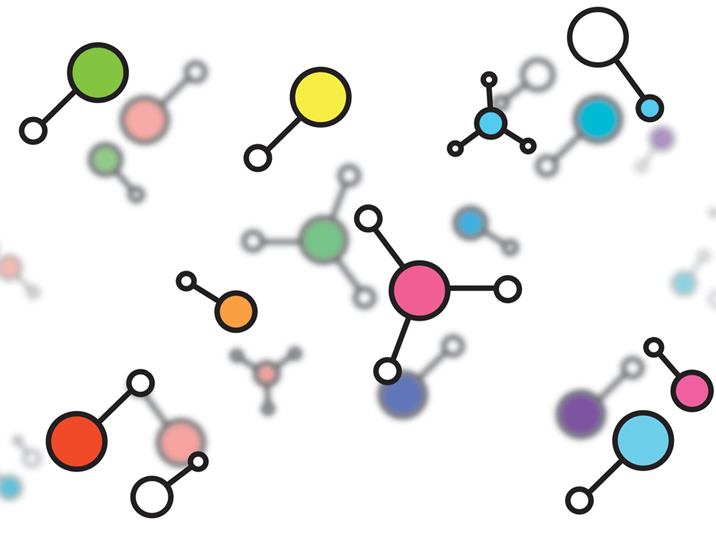
\includegraphics[	width=\paperwidth,
								height=\paperheight,keepaspectratio]
								{background.jpg}}
\end{frame}



\begin{frame}
\frametitle{Title}
{\scriptsize{}
	\tableofcontents
}
\end{frame}



\section{서론}

\subsection{목표}
\begin{frame}
\frametitle{목표}
{\scriptsize{}
	변수에 대한 정보만 존재하고 그들의 구조를 잘 모를 때 베이지안 네트워크 구조 학습을 진행하게 된다.
	
	{}\
	
	다양한 분야에서의 각 이론적 배경에 맞는 "적합한" 모형 선택을 돕기 위해,
	
	베이지안 네트워크의 구조 학습 방법을 선택하기 위한 여러가지 방법을 비교하고자 한다.
}
\end{frame}



\section{비교 기준}
\begin{frame}
\frametitle{Outline}
{\scriptsize{}
	\tableofcontents[currentsection]
}
\end{frame}



\subsection{비교 기준}
\begin{frame}
\frametitle{비교 기준}
{\scriptsize{}
	\begin{description}
	
	\item[점수를 이용한 비교] BDe, Log Likelihood, AIC, BIC
	
	주의! 점수가 "클수록" 좋다.(*1)

	\item[목표 네트워크와 학습된 네트워크와의 직접 비교(*2)]
	
		학습된 모형 자체가 실제 기대한 모형과 일치한지 자체에 주목한다.

		\begin{itemize}
			\item C (Correct Arcs) : 목표 네트워크 O, 학습 네트워크 O, 방향 일치
			\item M (Missing Arcs) : 목표 네트워크 O, 학습 네트워크에 X
			\item WO (Wrongly Oriented Arcs) : 목표 네트워크 O, 학습 네트워크 O, 방향 불일치
			\item WC (Wrolgly Connected Arcs) : 목표 네트워크 X, 학습 네트워크 O
		\end{itemize}
	\end{description}
}

{}\

\tiny{(*1) Silvia Acid 외 5명,

"A comparison of learning algorithms for Bayesian networks: a case study based on data from an emergency medical service",

Artificial Intelligence in Medicine 30 (2004) 215–232.}

{}\

\tiny{(*2) Reference : Fadhl, M. Al-Akwaa, Mohammed M. lkhawlani, (2012),

"Comparison of the Bayesian Network Structure Learning Algorithms",

International Journal of Advanced Research in Computer Science and Software Engineering Volume 2, Issue 3.}

\end{frame}



\subsection{어떻게 비교할 것인가?}
\begin{frame}
\frametitle{어떻게 비교할 것인가?}
{\scriptsize{}
	\begin{itemize}
		\item 어떤 Algorithm을 적용했는가에 따라
		
		\item Topology의 유형에 따라

		\item Node 개수가 증가함에 따라
	
		\item Sample Size가 증가함에 따라
	\end{itemize}
}
\end{frame}



\subsection{전제}
\begin{frame}
\frametitle{전제}
{\scriptsize{}
	\begin{itemize}
		\item 각 Node에 대한 Cardinality는 2로 제한한다.
		
		(즉, 이 모든 Node가 Binary Data인 경우만 다룬다.)
		
		\item 이 연구에서 사용하는 구조 학습 알고리즘은 R의 bnlearn 패키지에서 제공하는 것으로 한정한다.
		
		\item 모든 실험은 100번 반복하였다. 그 결과들을 받아 종합하였다.

		\item Synthetic Data로 분석할 때, 확률 관계를 정의할 때, 확률값을 U(0,1) 사이의 값에서 임의로 주었다.
	\end{itemize}
}
\end{frame}



\section{Real Data를 이용한 구조 학습 결과 비교}
\begin{frame}
\frametitle{Outline}
{\scriptsize{}
	\tableofcontents[currentsection]
}
\end{frame}


\subsection{Asia DataSet by Lauritzen and Spiegelhalter}
\begin{frame}
\frametitle{Asia DataSet}
{\scriptsize{}
\begin{description}
	\item[Description] Small synthetic data set from Lauritzen and Spiegelhalter (1988) about lung diseases (tuberculosis, lung cancer or bronchitis) and visits to Asia.
	
	\item[Number of nodes] 8
	
	\item[Number of arcs] 8
	
	\item[Number of parameters] 18
	
	\item[Source] Lauritzen S, Spiegelhalter D (1988).
	
	"Local Computation with Probabilities on Graphical Structures and their Application to Expert Systems (with discussion)".
	
	Journal of the Royal Statistical Society: Series B (Statistical Methodology), 50(2), 157-224.
\end{description}
}
\end{frame}


\begin{frame}
\frametitle{Asia DataSet}
{\scriptsize{}
	\begin{figure}
		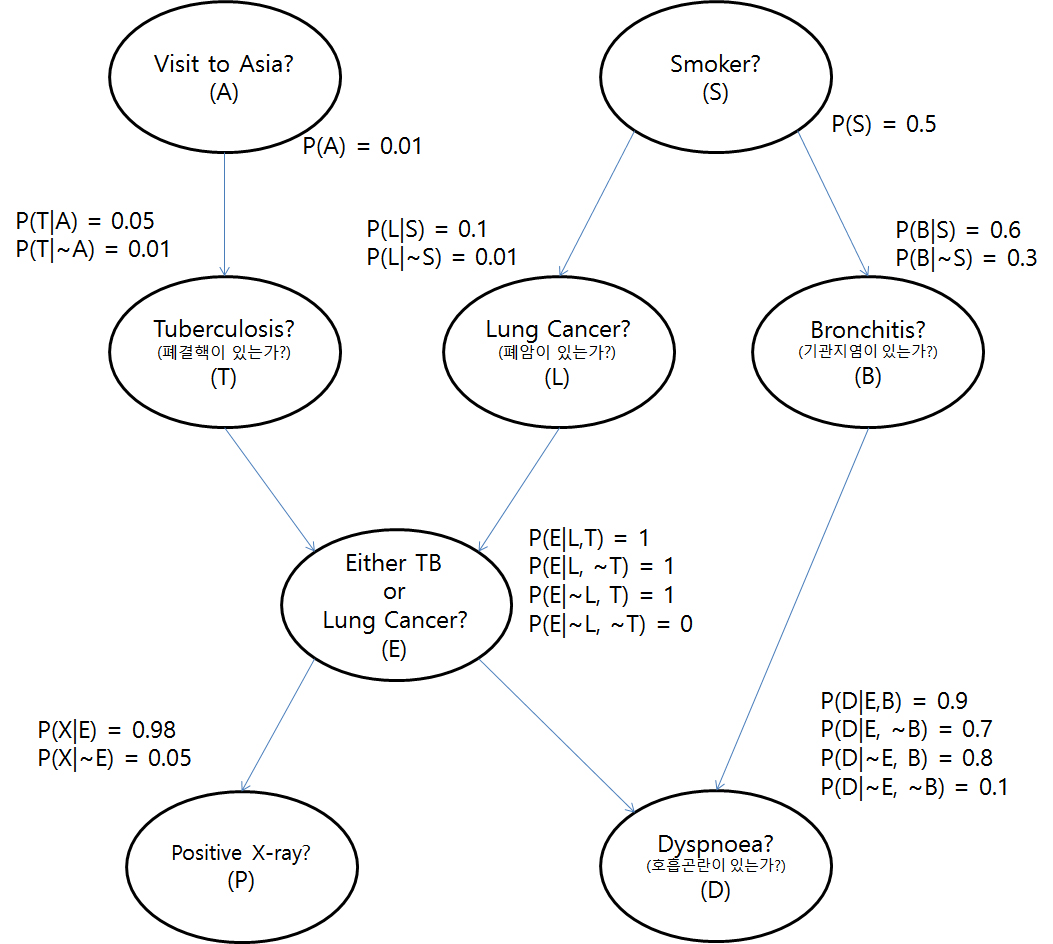
\includegraphics[height=170pt]{images/image01}
	\end{figure}	
}
\end{frame}



\begin{frame}
\frametitle{선행연구와 결과 비교 : Asia DataSet}
{\scriptsize{}
	\begin{figure}
		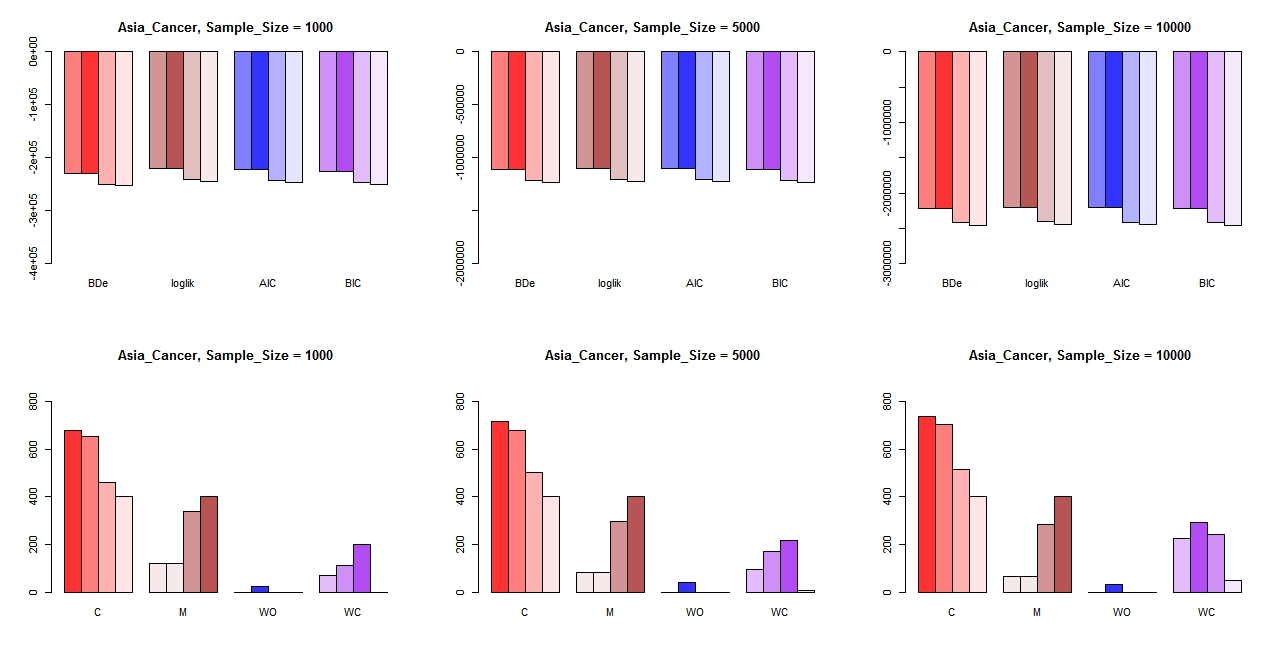
\includegraphics[height=170pt]{images/Real_1_Asia}
	\end{figure}	
}
\end{frame}



\subsection{Insurance Evaluation Network DataSet}
\begin{frame}
\frametitle{Insurance DataSet}
{\scriptsize{}
\begin{description}
	\item[Description] Insurance is a network for evaluating car insurance risks.
	
	\item[Number of nodes] 27
	
	\item[Number of arcs] 52
	
	\item[Number of parameters] 984
	
	\item[Source]  Binder J, Koller D, Russell S, Kanazawa K (1997).

	 "Adaptive Probabilistic Networks with Hidden Variables".
	 
	  Machine Learning, 29(2-3), 213-244.
\end{description}
}
\end{frame}


\begin{frame}
\frametitle{Insurance DataSet}
{\scriptsize{}
	\begin{figure}
		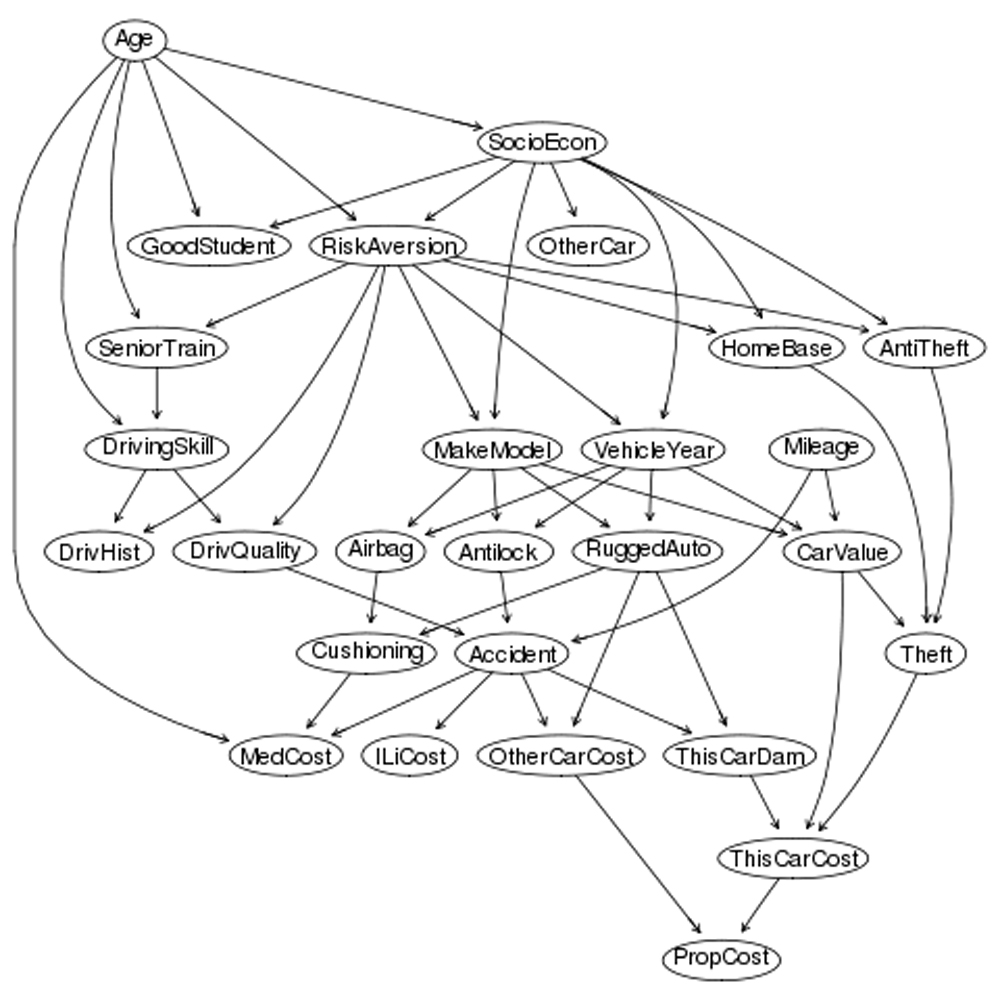
\includegraphics[height=170pt]{images/image02}
	\end{figure}	
}
\end{frame}


\begin{frame}
\frametitle{Insurance DataSet}
{\scriptsize{}
	\begin{figure}
		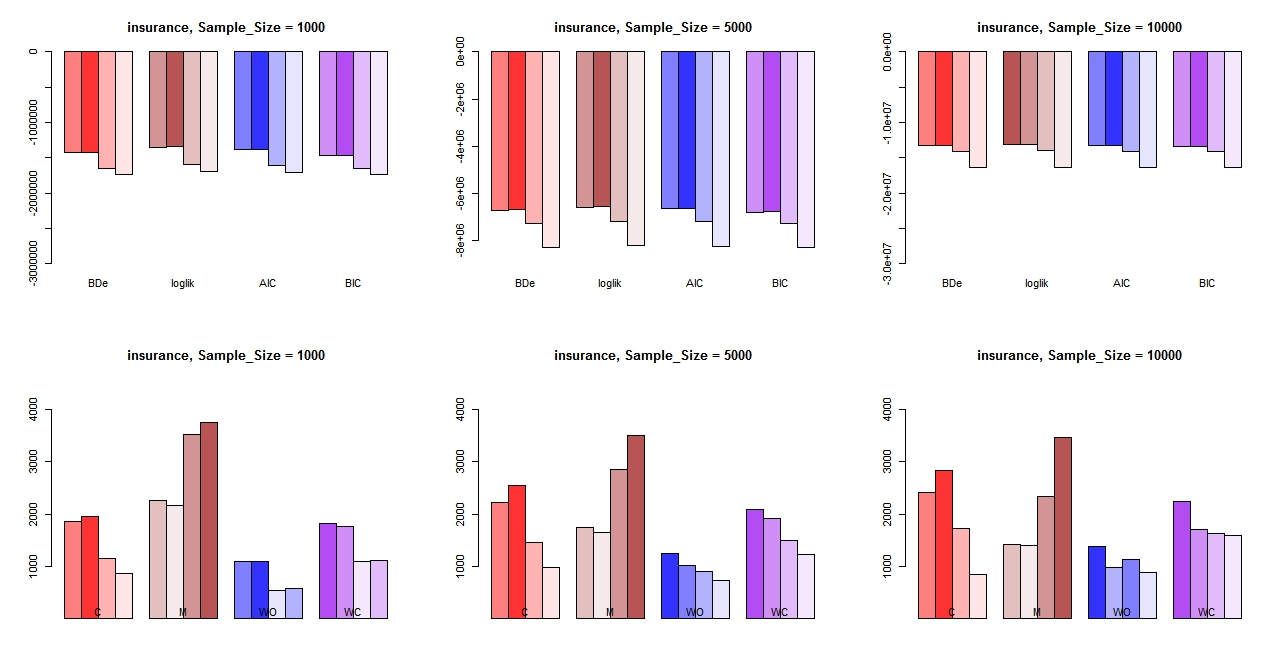
\includegraphics[height=170pt]{images/Real_2_Insurance}
	\end{figure}		
}
\end{frame}



\subsection{ALARM Monitoring System DataSet}
\begin{frame}
\frametitle{Alarm DataSet}
{\scriptsize{}
\begin{description}
	\item[Description] The ALARM ("A Logical Alarm Reduction Mechanism") is a Bayesian network designed to provide an alarm message system for patient monitoring.
	
	\item[Number of nodes] 37
	
	\item[Number of arcs] 46
	
	\item[Number of parameters] 509
	
	\item[Source]  Beinlich I, Suermondt HJ, Chavez RM, Cooper GF (1989).
	
	"The ALARM Monitoring System: A Case Study with Two Probabilistic Inference Techniques for Belief Networks."
	
	In "Proceedings of the 2nd European Conference on Artificial Intelligence in Medicine", pp. 247-256. Springer-Verlag.
\end{description}
}
\end{frame}


\begin{frame}
\frametitle{Alarm DataSet}
{\scriptsize{}
	\begin{figure}
		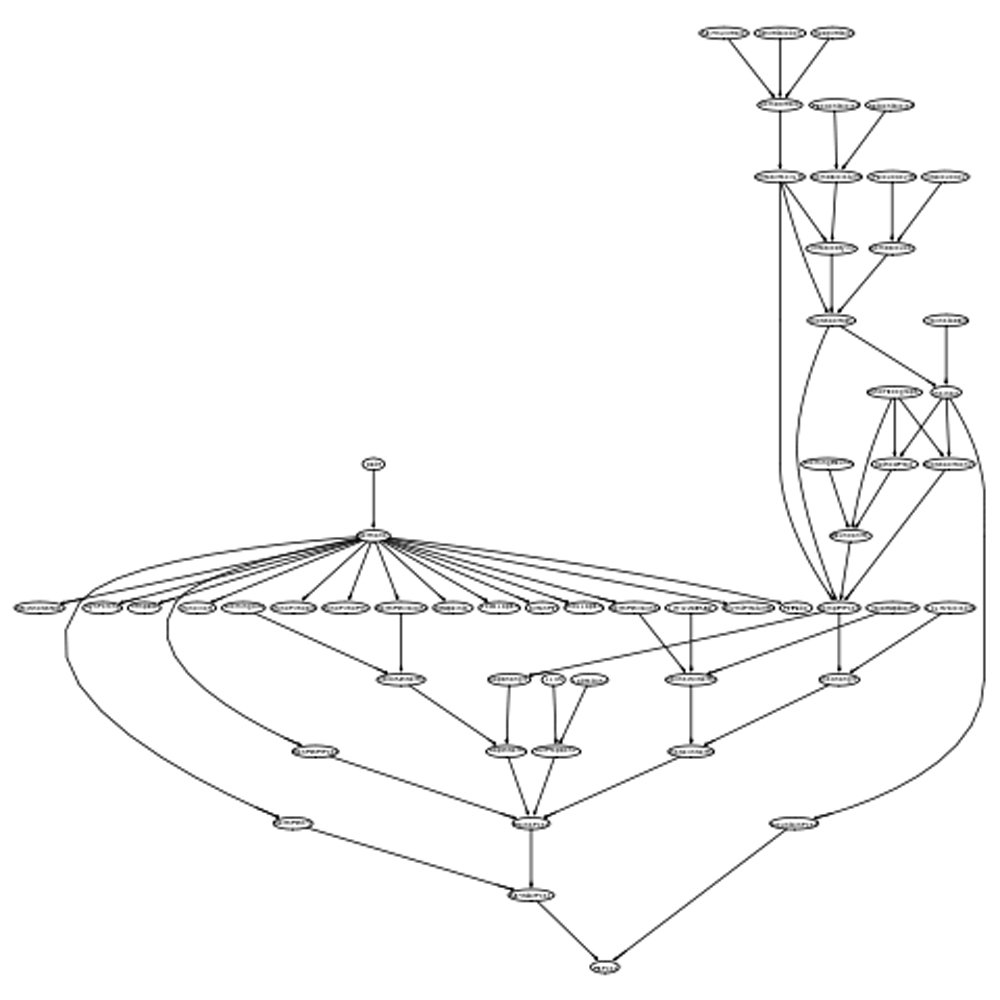
\includegraphics[height=170pt]{images/image03}
	\end{figure}	
}
\end{frame}


\begin{frame}
\frametitle{Alarm DataSet}
{\scriptsize{}
	\begin{figure}
		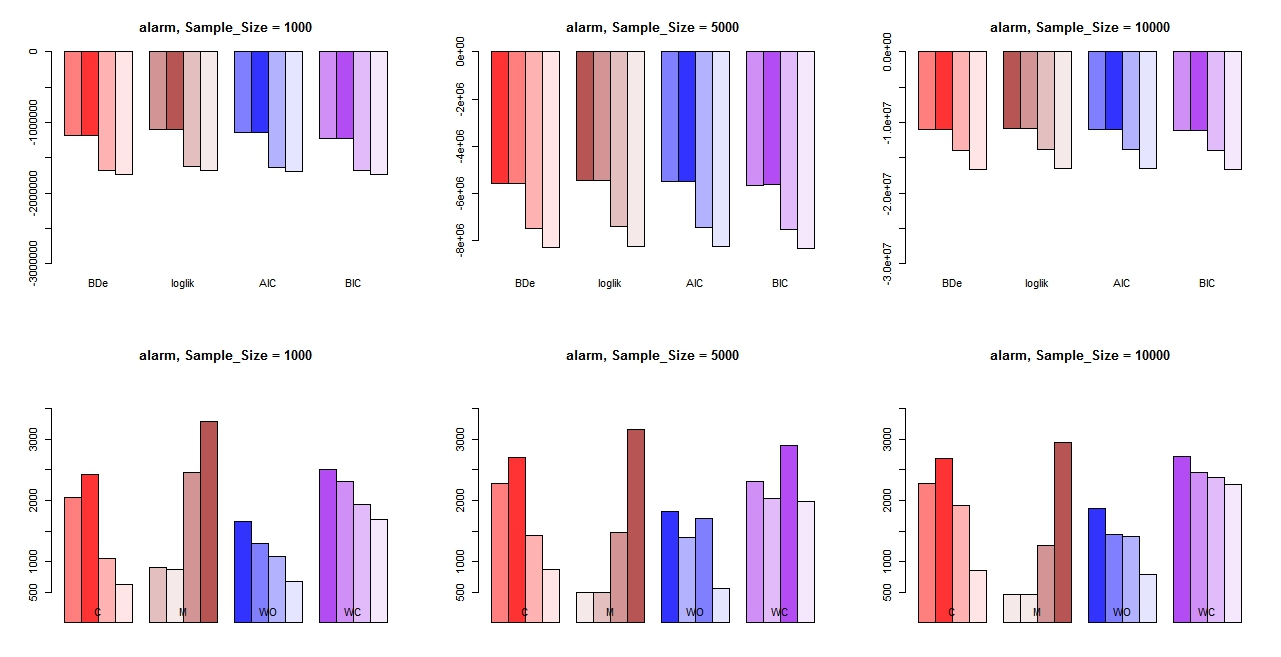
\includegraphics[height=170pt]{images/Real_3_Alarm}
	\end{figure}			
}
\end{frame}



\subsection{The HailFinder Weather Forecast System DataSet}
\begin{frame}
\frametitle{HailFinder DataSet}
{\scriptsize{}
\begin{description}
	\item[Description] Hailfinder is a Bayesian network designed to forecast severe summer hail in northeastern Colorado.
	
	\item[Number of nodes] 56
	
	\item[Number of arcs] 66
	
	\item[Number of parameters] 2656
	
	\item[Source]  Abramson B, Brown J, Edwards W, Murphy A, Winkler RL (1996).
	
	"Hailfinder: A Bayesian system for forecasting severe weather".
	
	International Journal of Forecasting, 12(1), 57-71.
\end{description}
}
\end{frame}


\begin{frame}
\frametitle{HailFinder DataSet}
{\scriptsize{}
	\begin{figure}
		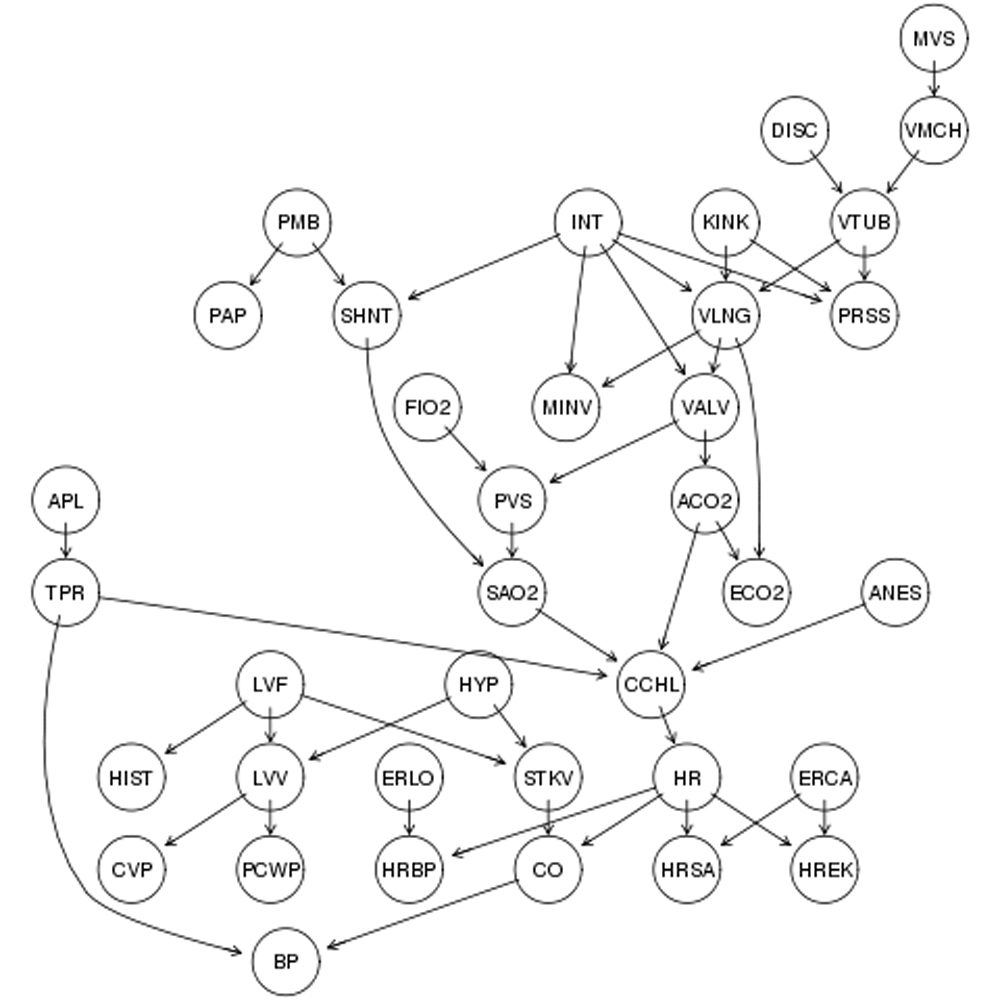
\includegraphics[height=170pt]{images/image04}
	\end{figure}	
}
\end{frame}


\begin{frame}
\frametitle{HailFinder DataSet}
{\scriptsize{}
		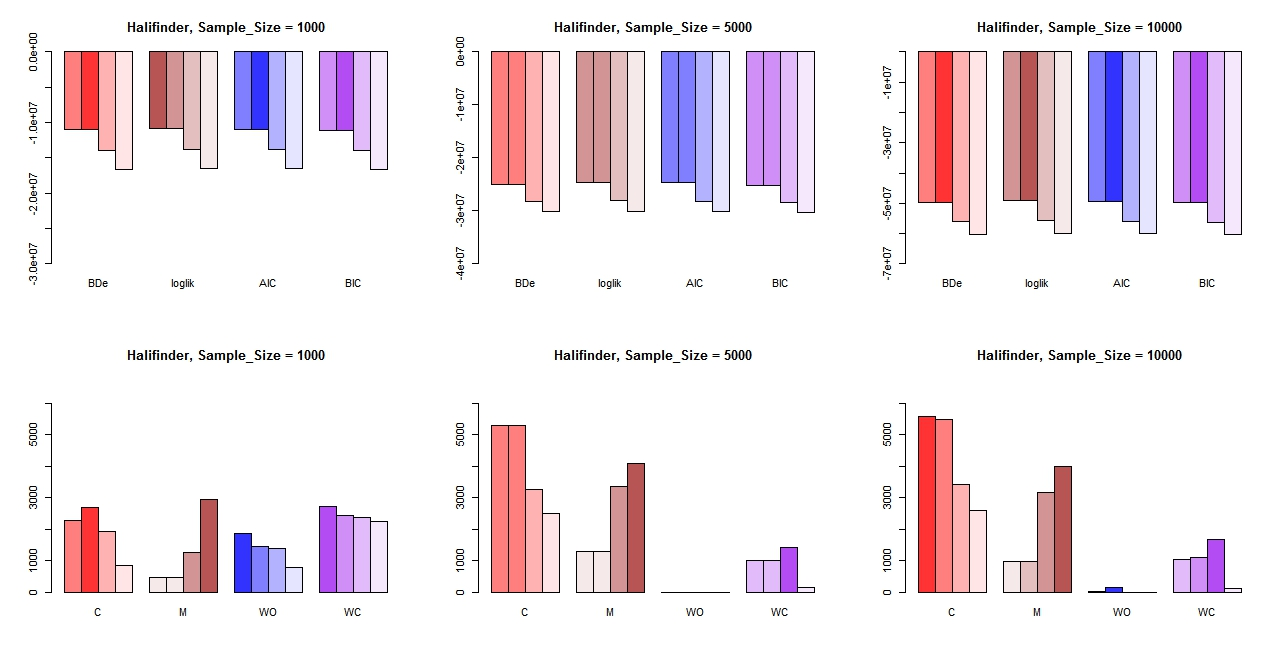
\includegraphics[height=170pt]{images/Real_4_Halifinder}
}
\end{frame}


\begin{frame}
\frametitle{Summary}
{\scriptsize{}
	\begin{center}
		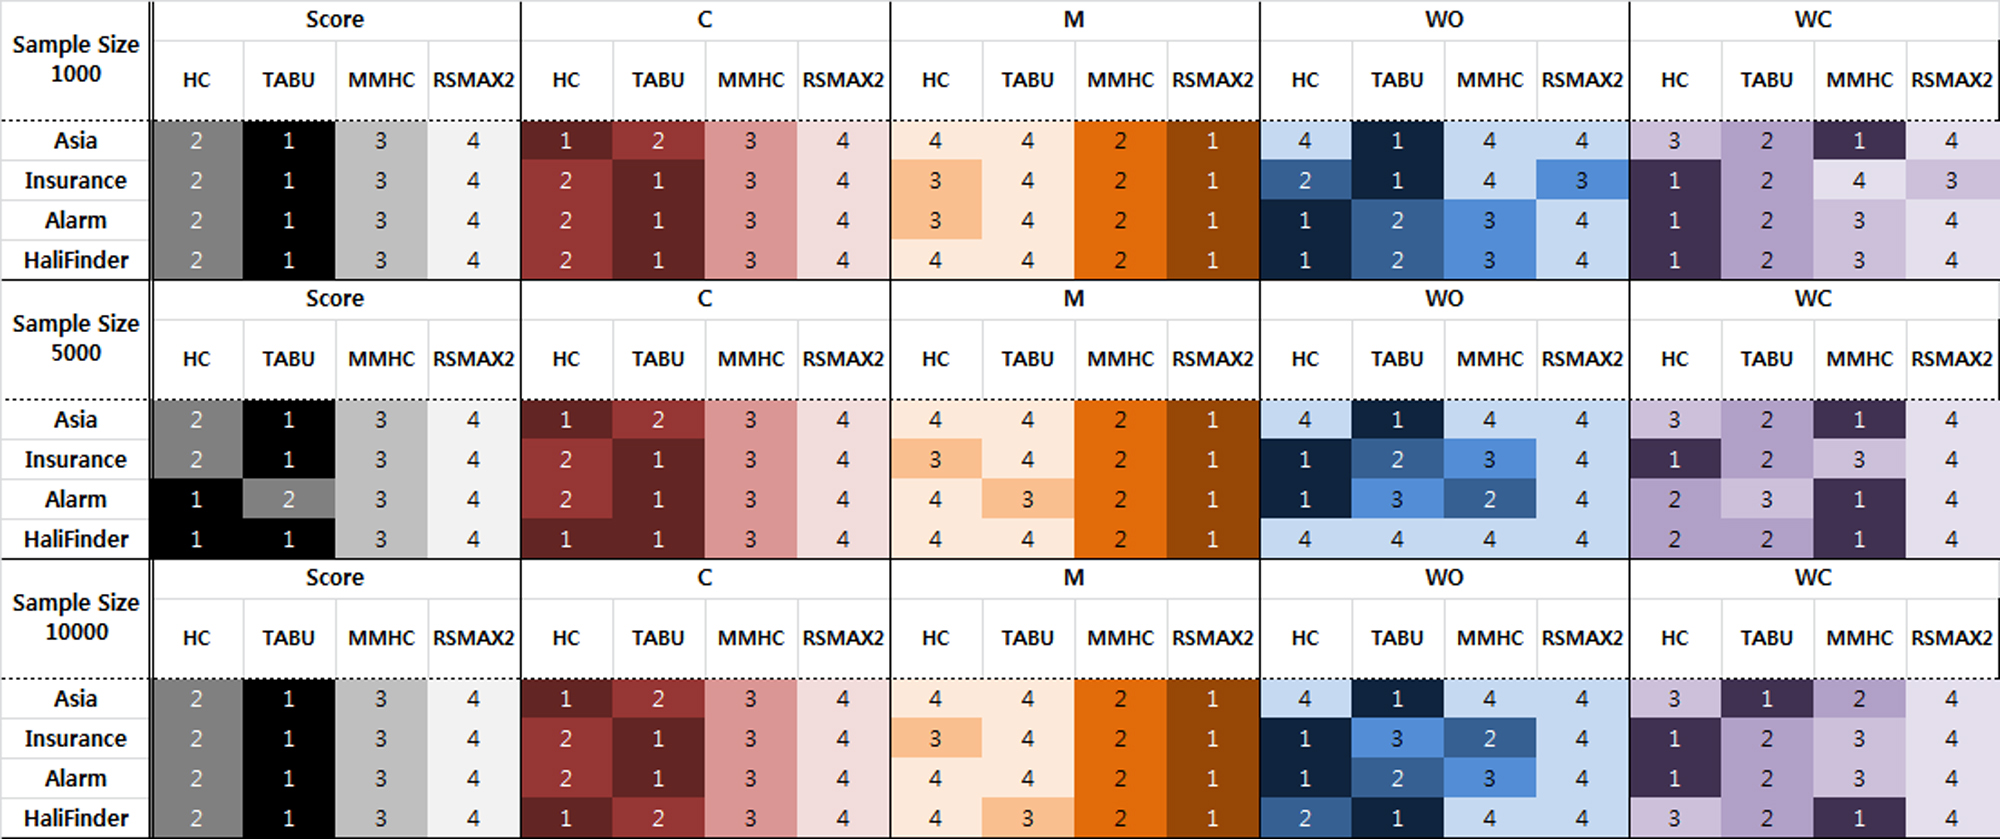
\includegraphics[height=130pt]{images/Real_Result}
	\end{center}
}
\end{frame}


\section{Data Generator 성능 평가}
\begin{frame}
\frametitle{Outline}
{\scriptsize{}
	\tableofcontents[currentsection]
}
\end{frame}


\begin{frame}
\frametitle{Data Generator 성능 평가}

{\scriptsize{}
	\textbf{BN$\_$Data$\_$Generator} $\{$User-Defined Function$\}$

	\begin{center}	
		베이지안 네트워크 데이터 생성기
	\end{center}
	
	\begin{description}
		\item[Description] 베이지안 네트워크 모형을 기반으로 Synthetic Data를 생성하여 준다.
		
		\item[Usage] BN$\_$Data$\_$Generator (arcs, input$\_$Probs, n, node$\_$names)
		
		\item[Arguments]
	\end{description}
	
	\begin{center}
				\begin{tabular}{c|c|c}
					\hline 
					\textbf{arcs} & (matrix) & 모형 내 arc 유무와 방향을 결정하는 행렬\tabularnewline
					\hline 
					\textbf{input$\_$Probs} & (list) & arc가 이어져있는 node간 관계의 조건부 확률\tabularnewline
					\hline 
					\textbf{n} & (constant) & Sample Size\tabularnewline
					\hline 
					\textbf{node$\_$names} & (vector) & Node의 이름\tabularnewline
					\hline 
				\end{tabular}
	\end{center}
}
\end{frame}


\begin{frame}
\frametitle{Data Generator 성능 평가}

{\scriptsize{}
	\begin{center}
		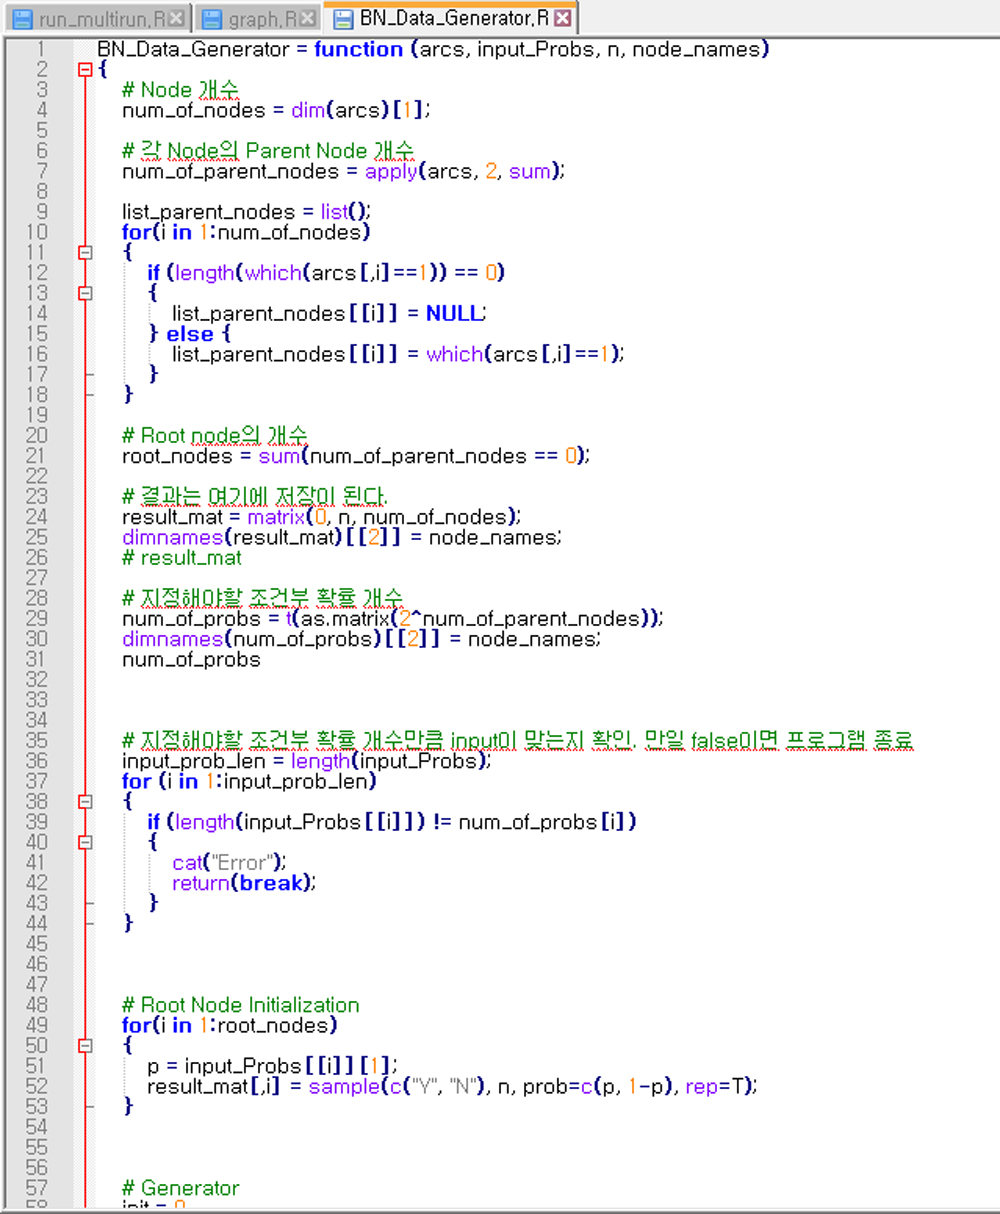
\includegraphics[height=170pt]{images/image22}
	\end{center}
}
\end{frame}


\begin{frame}
\frametitle{Data Generator 성능 평가}

{\scriptsize{}
	\begin{center}
		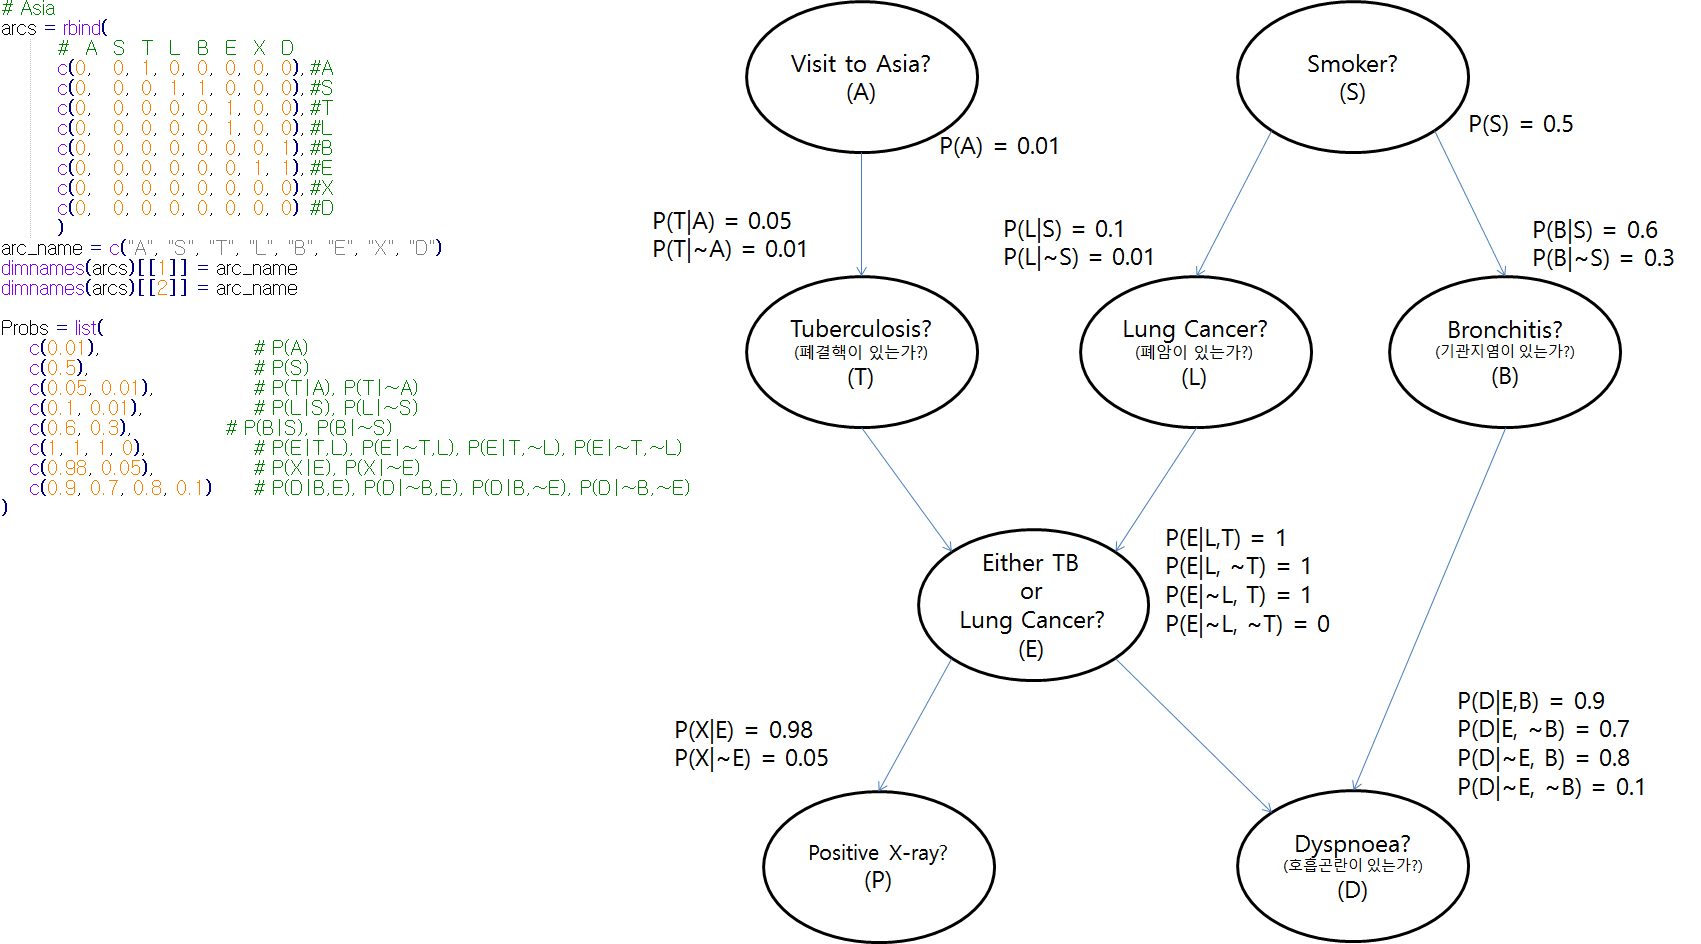
\includegraphics[height=170pt]{images/image24}
	\end{center}
}
\end{frame}


\begin{frame}
\frametitle{Data Generator 성능 평가}

{\scriptsize{}
	\begin{center}
		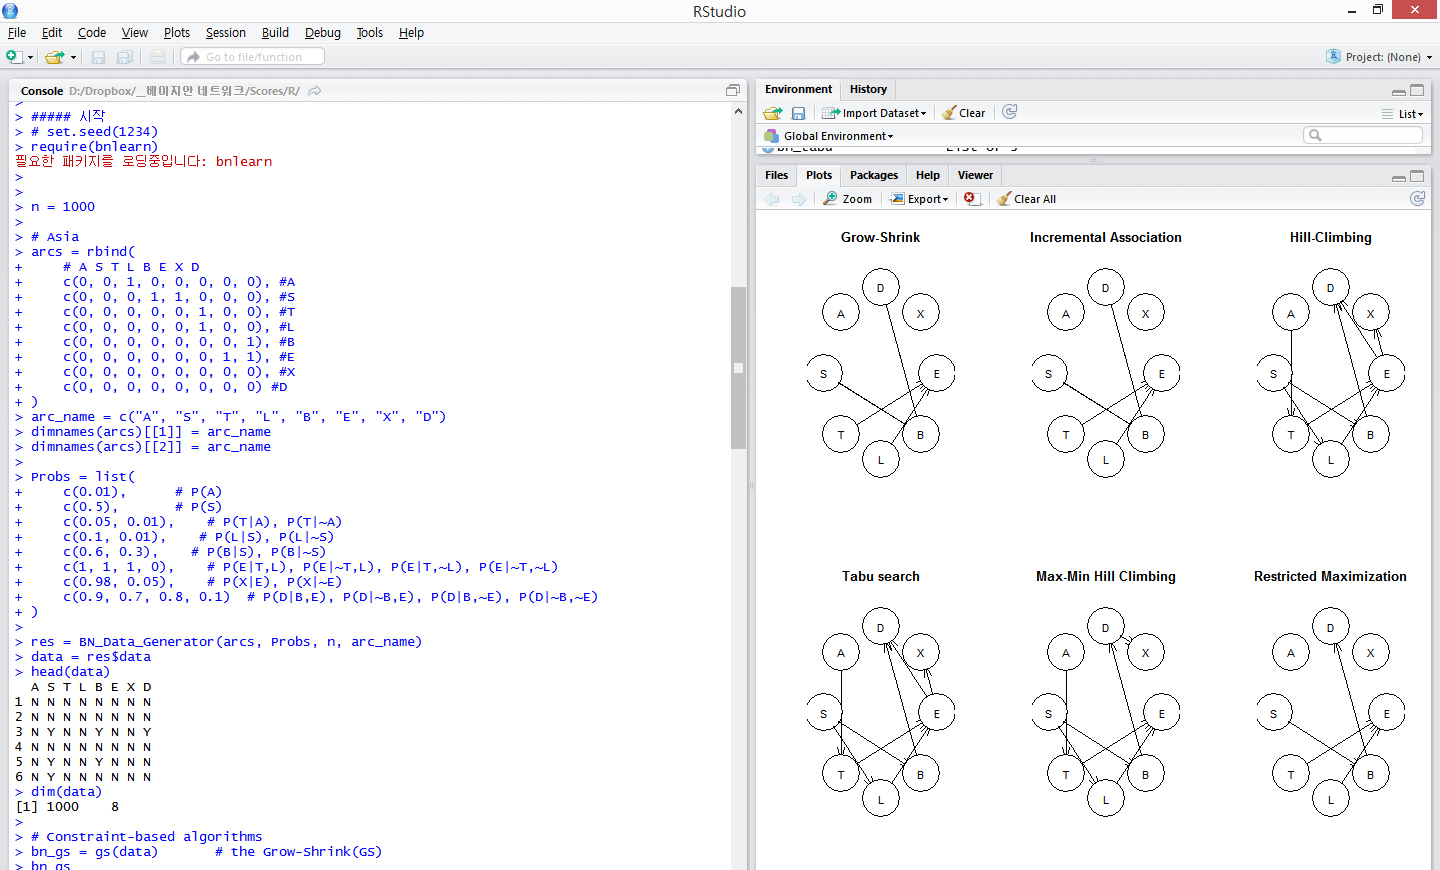
\includegraphics[height=170pt]{images/image23}
	\end{center}
}
\end{frame}



\begin{frame}
\frametitle{성능 평가를 위한 선행 연구}
{\scriptsize{}
Pekka Parviainen, Hossein Shahrabi Farahani, and Jens Lagergren (2014).

{}\

"Learning Bounded Tree-width Bayesian Networks using Integer Linear Programming"

{}\

Proceedings of the 17th International Conference on Artificial Intelligence and Statistics (AISTATS)
}
\end{frame}



\begin{frame}
\frametitle{Data Generator 성능 평가 via Hill Climbing (HC)}
{\scriptsize{}
\begin{center}

\begin{tabular}{c|c|c|r|r|r|r|r}
\hline 
\multirow{2}{*}{{\tiny{}Dataset}} & {\tiny{}Num. of} & {\tiny{}Sample} & {\tiny{}ILP} & \multicolumn{4}{c}{{\tiny{}Score via HC}}\tabularnewline
\cline{4-8} 
 & {\tiny{}Nodes} & {\tiny{}Size} & {\tiny{}BDe} & {\tiny{}BDe} & {\tiny{}loglik} & {\tiny{}AIC} & {\tiny{}BIC}\tabularnewline
\hline 
{\tiny{}Asia} & \multirow{9}{*}{{\tiny{}8}} & {\tiny{}100} & {\tiny{}-245.64} & {\tiny{}-251.07} & {\tiny{}-194.08} & {\tiny{}-210.08} & {\tiny{}-230.92}\tabularnewline
{\tiny{}real} &  & {\tiny{}1000} & {\tiny{}-2317.41} & {\tiny{}-2281.98} & {\tiny{}-2188.63} & {\tiny{}-2205.63} & {\tiny{}-2247.35}\tabularnewline
{\tiny{}dataset} &  & {\tiny{}10000} & {\tiny{}-22466.40} & {\tiny{}-21937.24} & {\tiny{}-21812.37} & {\tiny{}-21832.37} & {\tiny{}-21904.47}\tabularnewline
\cline{1-1} \cline{3-8} 
{\tiny{}Gen.} &  & {\tiny{}100} &  & {\tiny{}-271.30} & {\tiny{}-209.69} & {\tiny{}-222.69} & {\tiny{}-239.62}\tabularnewline
{\tiny{}by} &  & {\tiny{}1000} &  & {\tiny{}-2350.21} & {\tiny{}-2262.16} & {\tiny{}-2279.16} & {\tiny{}-2320.87}\tabularnewline
{\tiny{}WEKA} &  & {\tiny{}10000} &  & {\tiny{}-22529.57} & {\tiny{}-22419.24} & {\tiny{}-22437.24} & {\tiny{}-22502.14}\tabularnewline
\cline{1-1} \cline{3-8} 
{\tiny{}Gen.} &  & {\tiny{}100} &  & {\tiny{}-} & {\tiny{}-} & {\tiny{}-} & {\tiny{}-}\tabularnewline
{\tiny{}by} &  & {\tiny{}1000} &  & {\tiny{}-2289.26} & {\tiny{}-2197.43} & {\tiny{}-2214.43} & {\tiny{}-2256.15}\tabularnewline
{\tiny{}Generator} &  & {\tiny{}10000} &  & {\tiny{}-22521.67} & {\tiny{}-22403.53} & {\tiny{}-22420.53} & {\tiny{}-22481.82}\tabularnewline
\hline 
\end{tabular}

\end{center}
}
\end{frame}


\begin{frame}
\frametitle{Data Generator 성능 평가 via TABU Search}
{\scriptsize{}

\begin{center}
\begin{tabular}{c|c|c|r|r|r|r|r}
\hline 
\multirow{2}{*}{{\tiny{}Dataset}} & {\tiny{}Num. of} & {\tiny{}Sample} & {\tiny{}ILP} & \multicolumn{4}{c}{{\tiny{}Score via TABU}}\tabularnewline
\cline{4-8} 
 & {\tiny{}Nodes} & {\tiny{}Size} & {\tiny{}BDe} & {\tiny{}BDe} & {\tiny{}loglik} & {\tiny{}AIC} & {\tiny{}BIC}\tabularnewline
\hline 
{\tiny{}Asia} & \multirow{9}{*}{{\tiny{}8}} & {\tiny{}100} & {\tiny{}-245.64} & {\tiny{}-270.99} & {\tiny{}-206.14} & {\tiny{}-219.14} & {\tiny{}-236.08}\tabularnewline
{\tiny{}real} &  & {\tiny{}1000} & {\tiny{}-2317.41} & {\tiny{}-2342.17} & {\tiny{}-2249.24} & {\tiny{}-2266.24} & {\tiny{}-2307.96}\tabularnewline
{\tiny{}dataset} &  & {\tiny{}10000} & {\tiny{}-22466.40} & {\tiny{}-21996.98} & {\tiny{}-21870.55} & {\tiny{}-21889.55} & {\tiny{}-21958.05}\tabularnewline
\cline{1-1} \cline{3-8} 
{\tiny{}Gen.} &  & {\tiny{}100} &  & {\tiny{}-270.74} & {\tiny{}-208.81} & {\tiny{}-221.81} & {\tiny{}-238.74}\tabularnewline
{\tiny{}by} &  & {\tiny{}1000} &  & {\tiny{}-2350.21} & {\tiny{}-2262.16} & {\tiny{}-2279.16} & {\tiny{}-2320.87}\tabularnewline
{\tiny{}WEKA} &  & {\tiny{}10000} &  & {\tiny{}-22529.57} & {\tiny{}-22419.24} & {\tiny{}-22437.24} & {\tiny{}-22502.14}\tabularnewline
\cline{1-1} \cline{3-8} 
{\tiny{}Gen.} &  & {\tiny{}100} &  & {\tiny{}-} & {\tiny{}-} & {\tiny{}-} & {\tiny{}-}\tabularnewline
{\tiny{}by} &  & {\tiny{}1000} &  & {\tiny{}-2289.26} & {\tiny{}-2197.43} & {\tiny{}-2214.43} & {\tiny{}-2256.15}\tabularnewline
{\tiny{}Generator} &  & {\tiny{}10000} &  & {\tiny{}-22521.67} & {\tiny{}-22403.53} & {\tiny{}-22420.53} & {\tiny{}-22481.82}\tabularnewline
\hline 
\end{tabular}

\end{center}
}
\end{frame}


\begin{frame}
\frametitle{Data Generator 성능 평가 via MMHC}
{\scriptsize{}

\begin{center}
\begin{tabular}{c|c|c|r|r|r|r|r}
\hline 
\multirow{2}{*}{{\tiny{}Dataset}} & {\tiny{}Num. of} & {\tiny{}Sample} & {\tiny{}ILP} & \multicolumn{4}{c}{{\tiny{}Score via MMHC}}\tabularnewline
\cline{4-8} 
 & {\tiny{}Nodes} & {\tiny{}Size} & {\tiny{}BDe} & {\tiny{}BDe} & {\tiny{}loglik} & {\tiny{}AIC} & {\tiny{}BIC}\tabularnewline
\hline 
{\tiny{}Asia} & \multirow{9}{*}{{\tiny{}8}} & {\tiny{}100} & {\tiny{}-245.64} & {\tiny{}-301.29} & {\tiny{}-246.32} & {\tiny{}-257.32} & {\tiny{}-271.65}\tabularnewline
{\tiny{}real} &  & {\tiny{}1000} & {\tiny{}-2317.41} & {\tiny{}-2504.74} & {\tiny{}-2421.80} & {\tiny{}-2436.80} & {\tiny{}-2473.61}\tabularnewline
{\tiny{}dataset} &  & {\tiny{}10000} & {\tiny{}-22466.40} & {\tiny{}-24346.08} & {\tiny{}-24232.89} & {\tiny{}-24249.89} & {\tiny{}-24311.18}\tabularnewline
\cline{1-1} \cline{3-8} 
{\tiny{}Gen.} &  & {\tiny{}100} &  & {\tiny{}-272.31} & {\tiny{}-213.08} & {\tiny{}-225.08} & {\tiny{}-240.71}\tabularnewline
{\tiny{}by} &  & {\tiny{}1000} &  & {\tiny{}-2508.05} & {\tiny{}-2423.51} & {\tiny{}-2439.51} & {\tiny{}-2478.77}\tabularnewline
{\tiny{}WEKA} &  & {\tiny{}10000} &  & {\tiny{}-22815.07} & {\tiny{}-22709.96} & {\tiny{}-22725.96} & {\tiny{}-22783.64}\tabularnewline
\cline{1-1} \cline{3-8} 
{\tiny{}Gen.} &  & {\tiny{}100} &  & {\tiny{}-} & {\tiny{}-} & {\tiny{}-} & {\tiny{}-}\tabularnewline
{\tiny{}by} &  & {\tiny{}1000} &  & {\tiny{}-2446.05} & {\tiny{}-2360.82} & {\tiny{}-2376.82} & {\tiny{}-2416.08}\tabularnewline
{\tiny{}Generator} &  & {\tiny{}10000} &  & {\tiny{}-24137.75} & {\tiny{}-24026.34} & {\tiny{}-24042.34} & {\tiny{}-24100.02}\tabularnewline
\hline 
\end{tabular}
\end{center}
}
\end{frame}


\begin{frame}
\frametitle{Data Generator 성능 평가 via RSMAX2}
{\scriptsize{}

\begin{center}
\begin{tabular}{c|c|c|r|r|r|r|r}
\hline 
\multirow{2}{*}{{\tiny{}Dataset}} & {\tiny{}Num. of} & {\tiny{}Sample} & {\tiny{}ILP} & \multicolumn{4}{c}{{\tiny{}Score via RSMAX2}}\tabularnewline
\cline{4-8} 
 & {\tiny{}Nodes} & {\tiny{}Size} & {\tiny{}BDe} & {\tiny{}BDe} & {\tiny{}loglik} & {\tiny{}AIC} & {\tiny{}BIC}\tabularnewline
\hline 
{\tiny{}Asia} & \multirow{9}{*}{{\tiny{}8}} & {\tiny{}100} & {\tiny{}-245.64} & {\tiny{}-299.97} & {\tiny{}-246.07} & {\tiny{}-260.07} & {\tiny{}-278.31}\tabularnewline
{\tiny{}real} &  & {\tiny{}1000} & {\tiny{}-2317.41} & {\tiny{}-2531.66} & {\tiny{}-2451.91} & {\tiny{}-2464.91} & {\tiny{}-2496.81}\tabularnewline
{\tiny{}dataset} &  & {\tiny{}10000} & {\tiny{}-22466.40} & {\tiny{}-24295.92} & {\tiny{}-24194.06} & {\tiny{}-24207.06} & {\tiny{}-24253.93}\tabularnewline
\cline{1-1} \cline{3-8} 
{\tiny{}Gen.} &  & {\tiny{}100} &  & {\tiny{}-272.31} & {\tiny{}-213.08} & {\tiny{}-225.08} & {\tiny{}-240.71}\tabularnewline
{\tiny{}by} &  & {\tiny{}1000} &  & {\tiny{}-2534.36} & {\tiny{}-2456.36} & {\tiny{}-2469.36} & {\tiny{}-2501.26}\tabularnewline
{\tiny{}WEKA} &  & {\tiny{}10000} &  & {\tiny{}-22823.55} & {\tiny{}-22715.80} & {\tiny{}-22730.80} & {\tiny{}-22784.88}\tabularnewline
\cline{1-1} \cline{3-8} 
{\tiny{}Gen.} &  & {\tiny{}100} &  & {\tiny{}-} & {\tiny{}-} & {\tiny{}-} & {\tiny{}-}\tabularnewline
{\tiny{}by} &  & {\tiny{}1000} &  & {\tiny{}-2479.98} & {\tiny{}-2401.17} & {\tiny{}-2414.17} & {\tiny{}-2446.07}\tabularnewline
{\tiny{}Generator} &  & {\tiny{}10000} &  & {\tiny{}-24504.43} & {\tiny{}-24403.62} & {\tiny{}-24416.62} & {\tiny{}-24463.49}\tabularnewline
\hline 
\end{tabular}
\end{center}

}
\end{frame}



\section{Topology에 따른 비교}
\begin{frame}
\frametitle{Outline}
{\scriptsize{}
	\tableofcontents[currentsection]
}
\end{frame}


\begin{frame}
\frametitle{Topology에 따른 비교}
{\scriptsize{}
	\begin{center}
		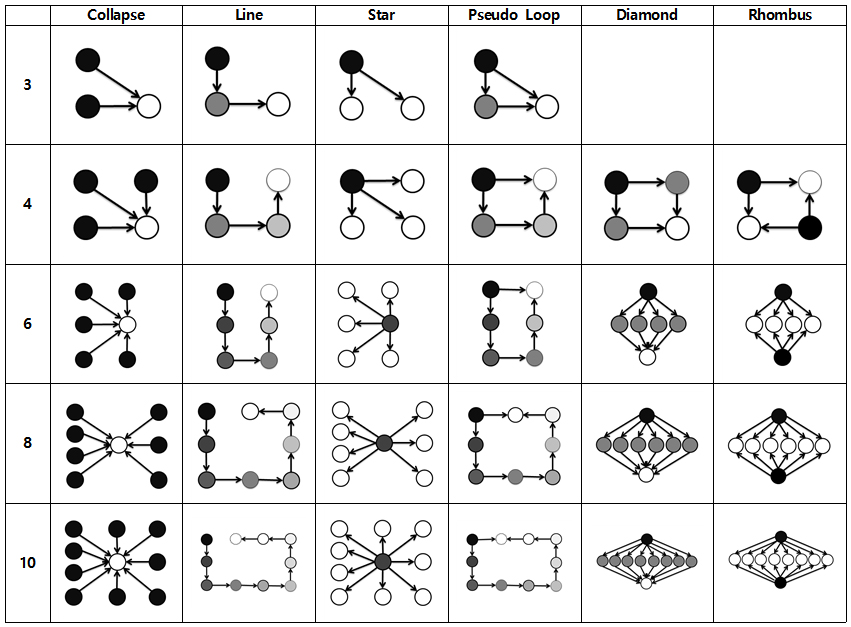
\includegraphics[height=150pt]{images/image21}
	\end{center}		
}
\tiny{
		Eitel J. M. Lauría,
		
		"An Information-Geometric Approach to Learning Bayesian Network Topologies from Data",
		
		Innovations in Bayesian Networks Studies in Computational Intelligence Volume 156, 2008, pp 187-217
		}
\end{frame}


\begin{frame}
\frametitle{Topology에 따른 비교 분석 : Collapse}
{\scriptsize{}
	\begin{figure}
		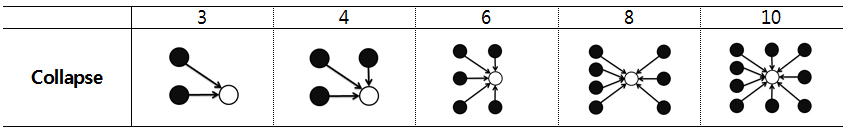
\includegraphics[height=50pt]{images/Topologies_Collapse}
	\end{figure}	
}
\end{frame}



\begin{frame}
\frametitle{Topology에 따른 비교 : Collapse (Score)}
{\scriptsize{}
	\begin{figure}
		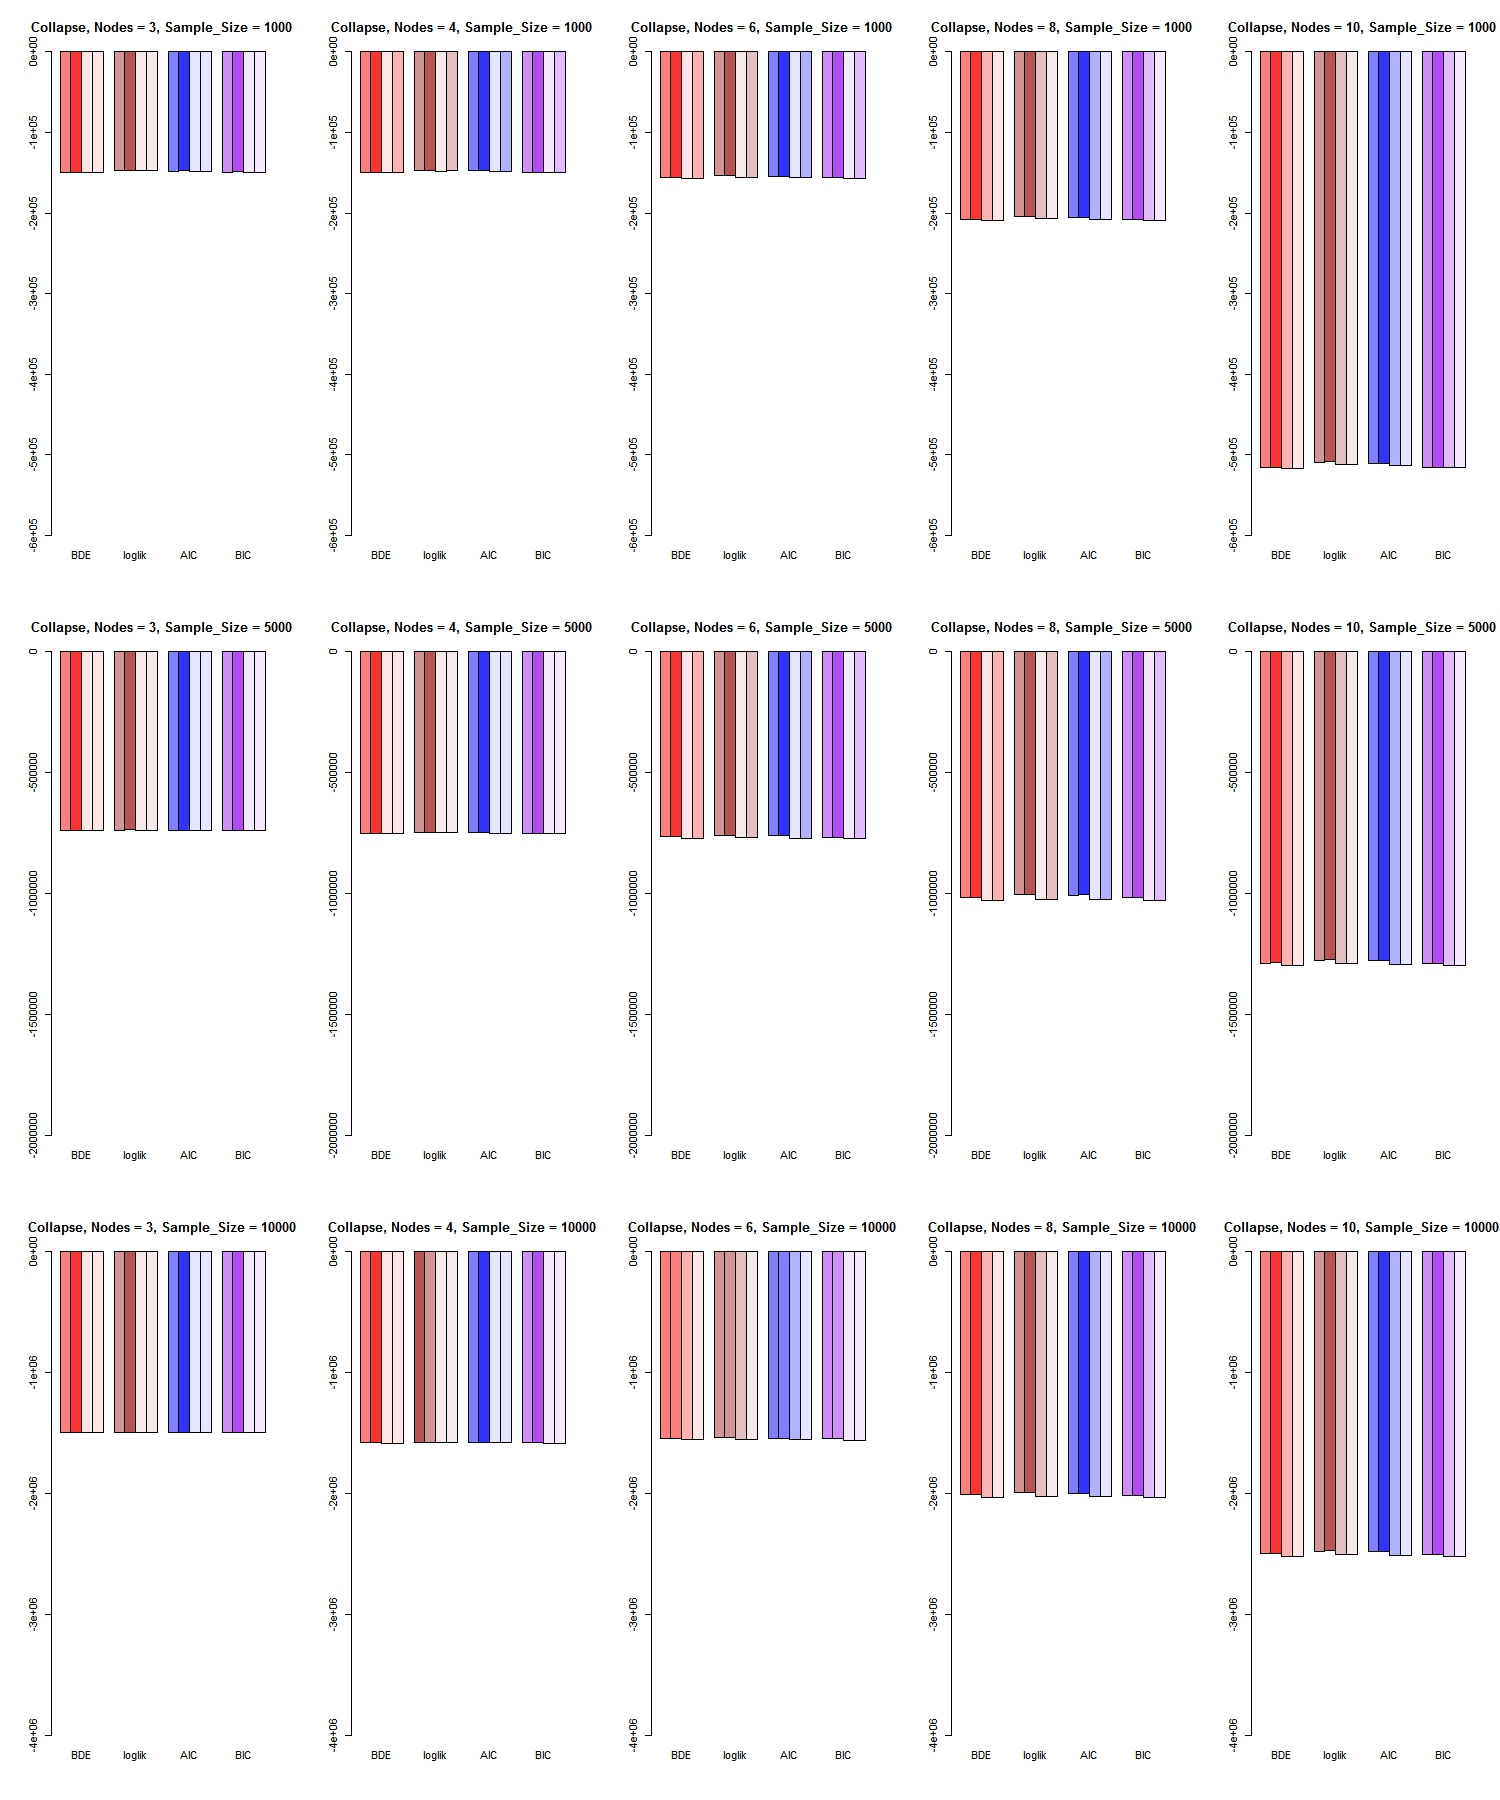
\includegraphics[height=170pt]{images/01_Collapse_Score}
	\end{figure}	
}
\end{frame}


\begin{frame}
\frametitle{Topology에 따른 비교 : Collapse (Arcs)}
{\scriptsize{}
	\begin{figure}
		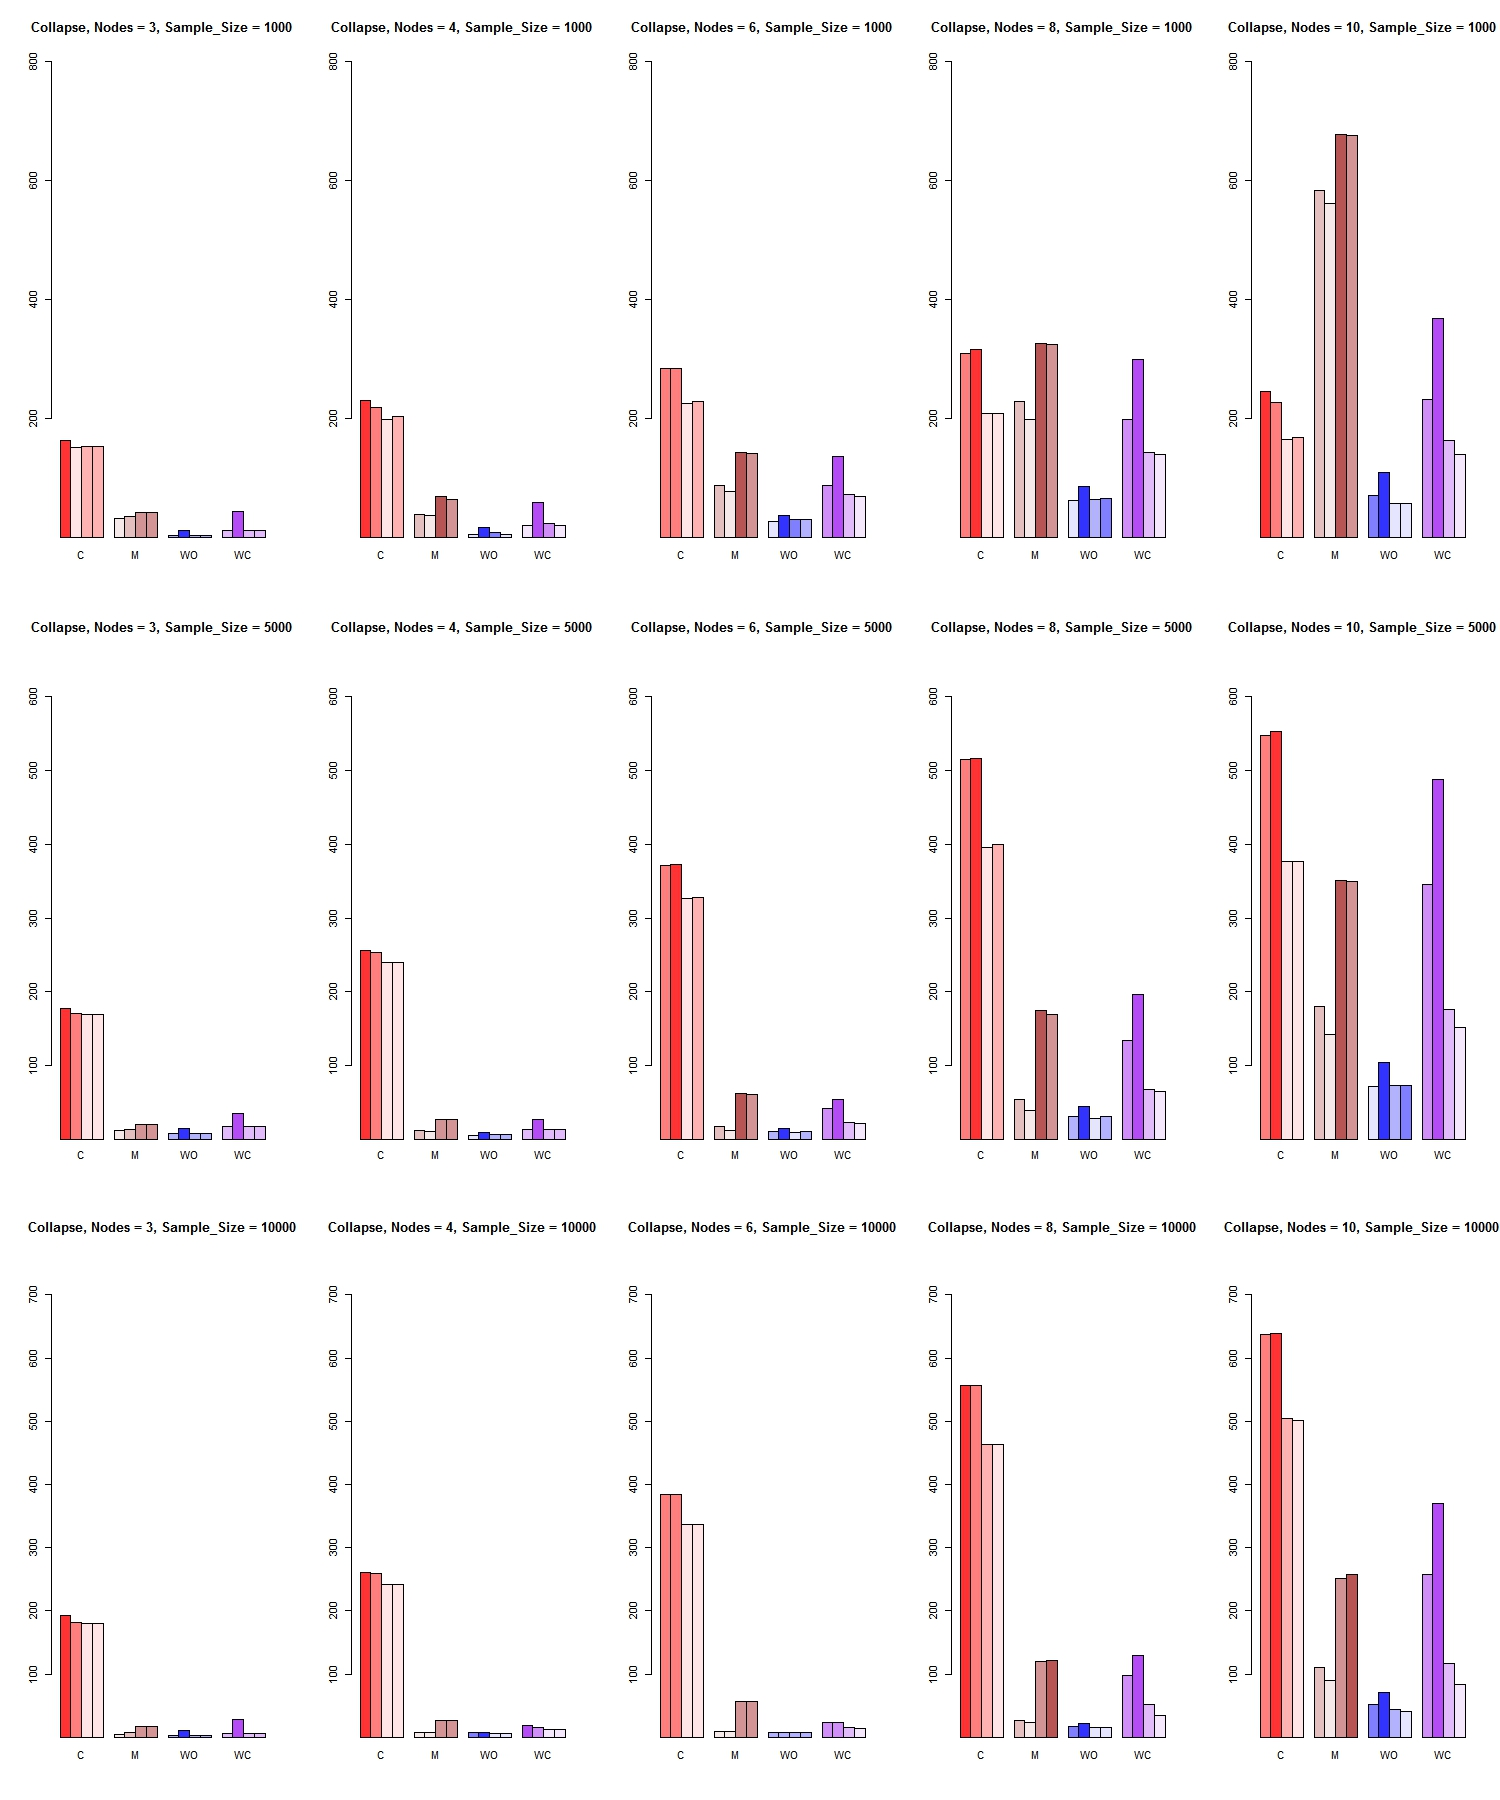
\includegraphics[height=170pt]{images/01_Collapse_Arcs}
	\end{figure}	
}
\end{frame}



\begin{frame}
\frametitle{Topology에 따른 비교 : Collapse}
{\scriptsize{}
	\begin{center}
		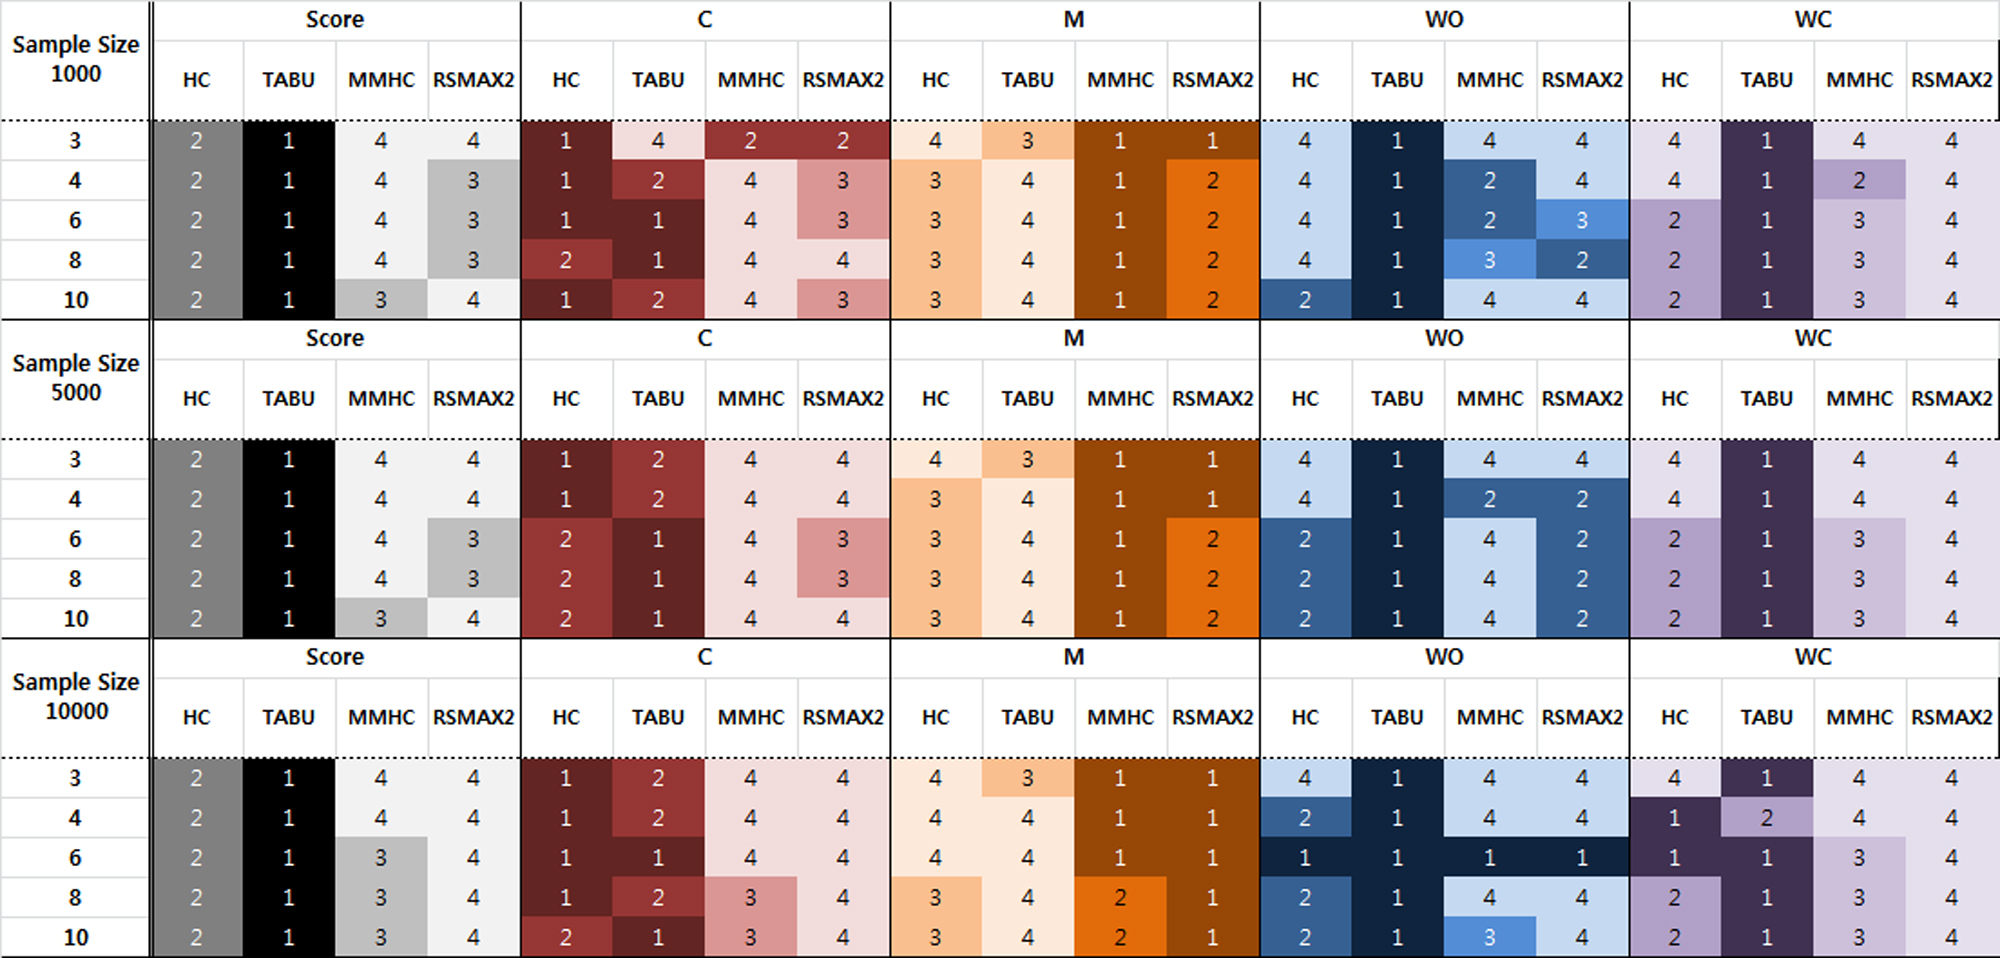
\includegraphics[height=130pt]{images/Result_Collapse}
	\end{center}
}
\end{frame}



\begin{frame}
\frametitle{Topology에 따른 비교 분석 : Line}
{\scriptsize{}
	\begin{figure}
		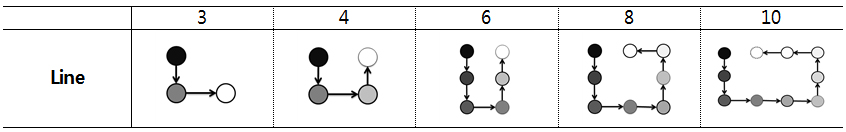
\includegraphics[height=50pt]{images/Topologies_Line}
	\end{figure}	
}
\end{frame}



\begin{frame}
\frametitle{Topology에 따른 비교 : Line (Score)}
{\scriptsize{}
	\begin{figure}
		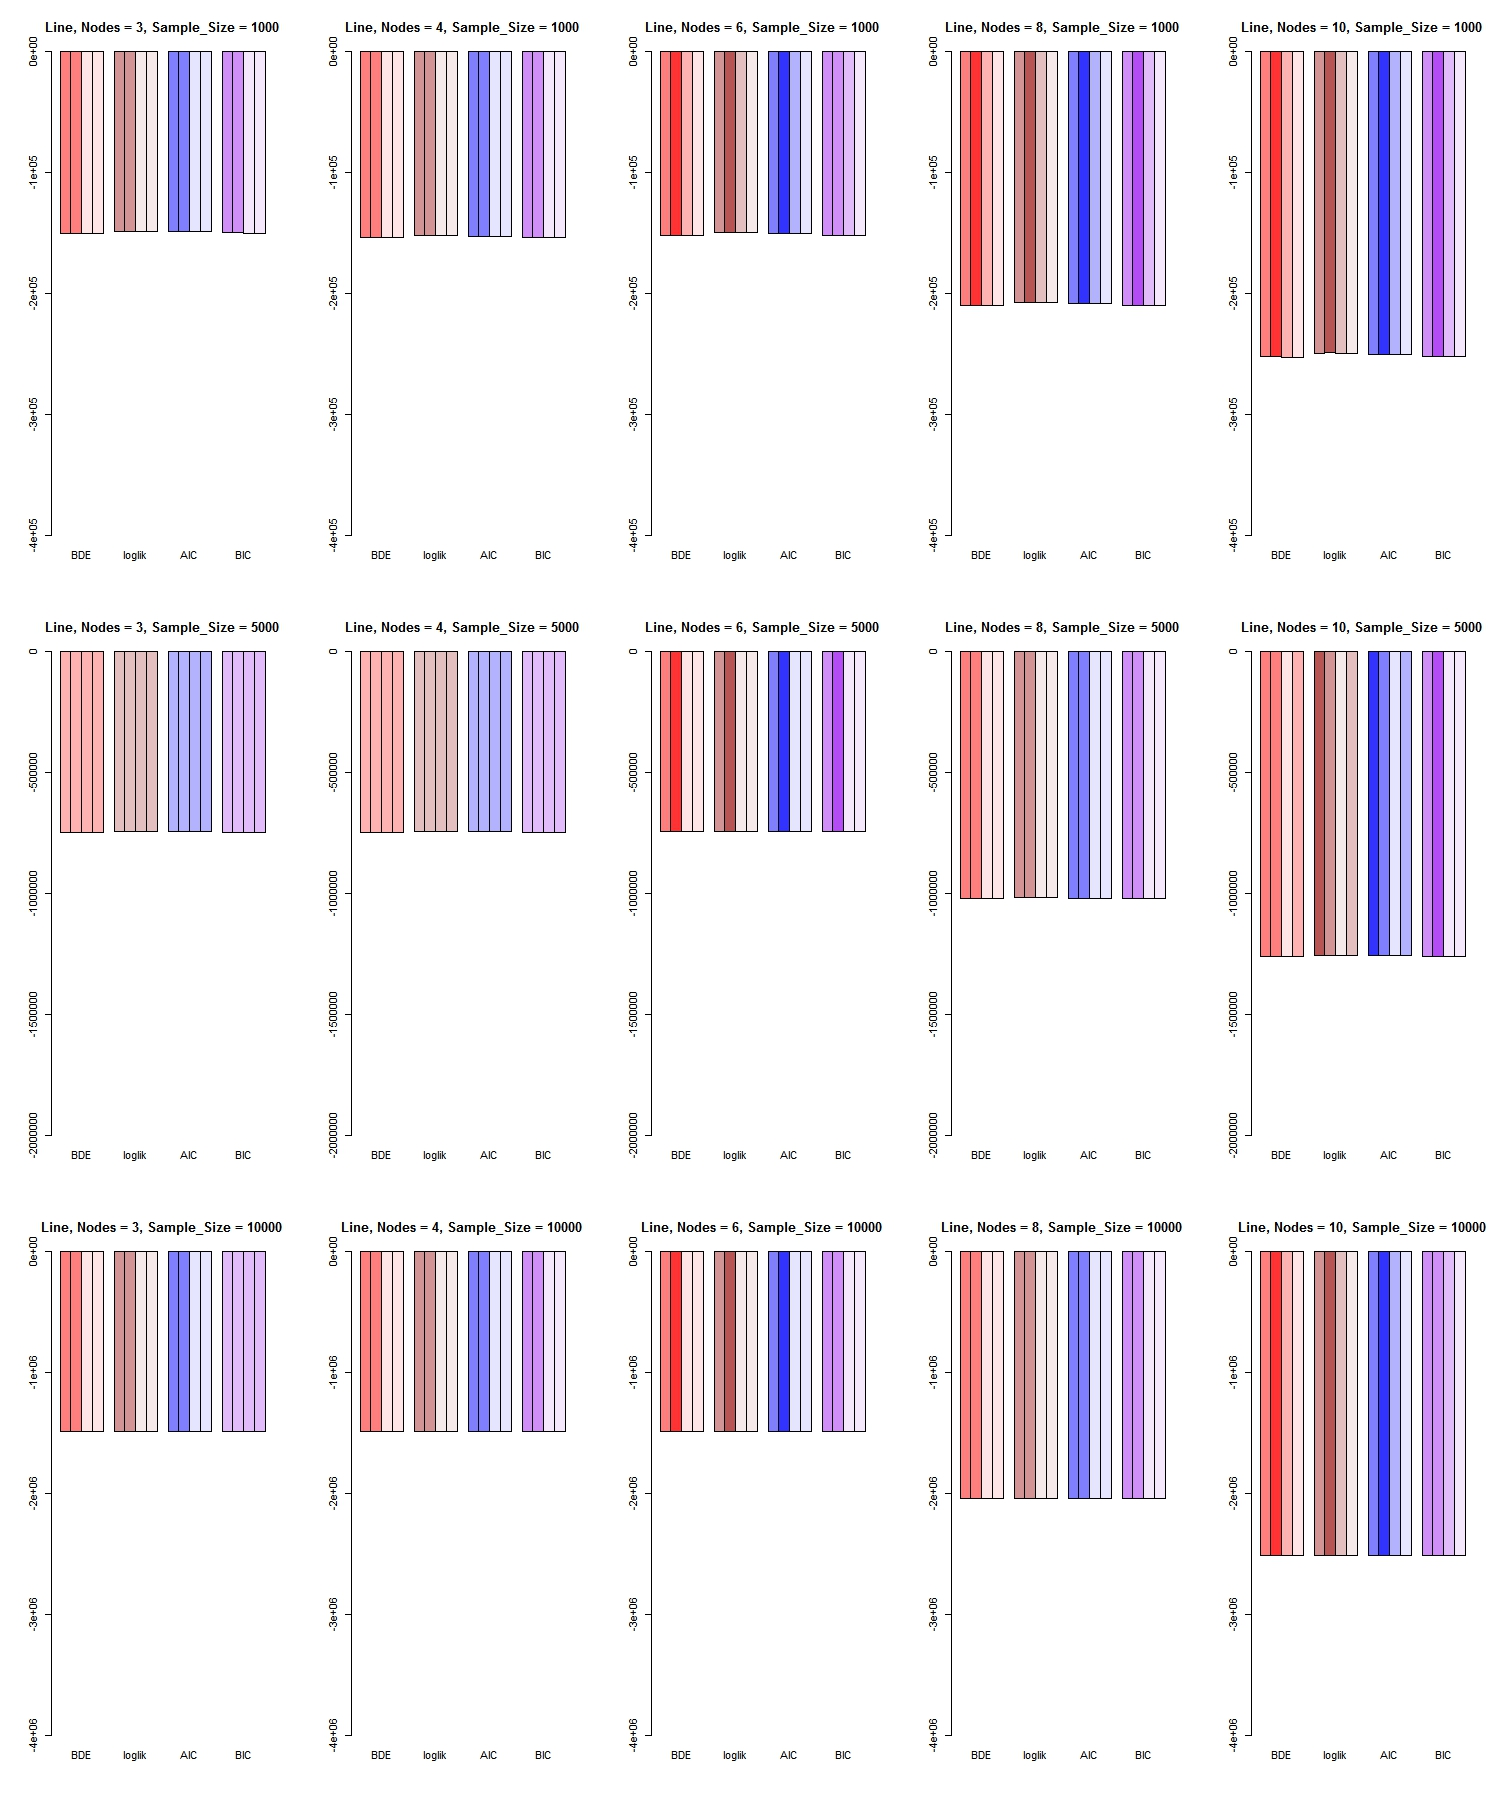
\includegraphics[height=170pt]{images/02_Line_Score}
	\end{figure}	
}
\end{frame}


\begin{frame}
\frametitle{Topology에 따른 비교 : Line (Arcs)}
{\scriptsize{}
	\begin{figure}
		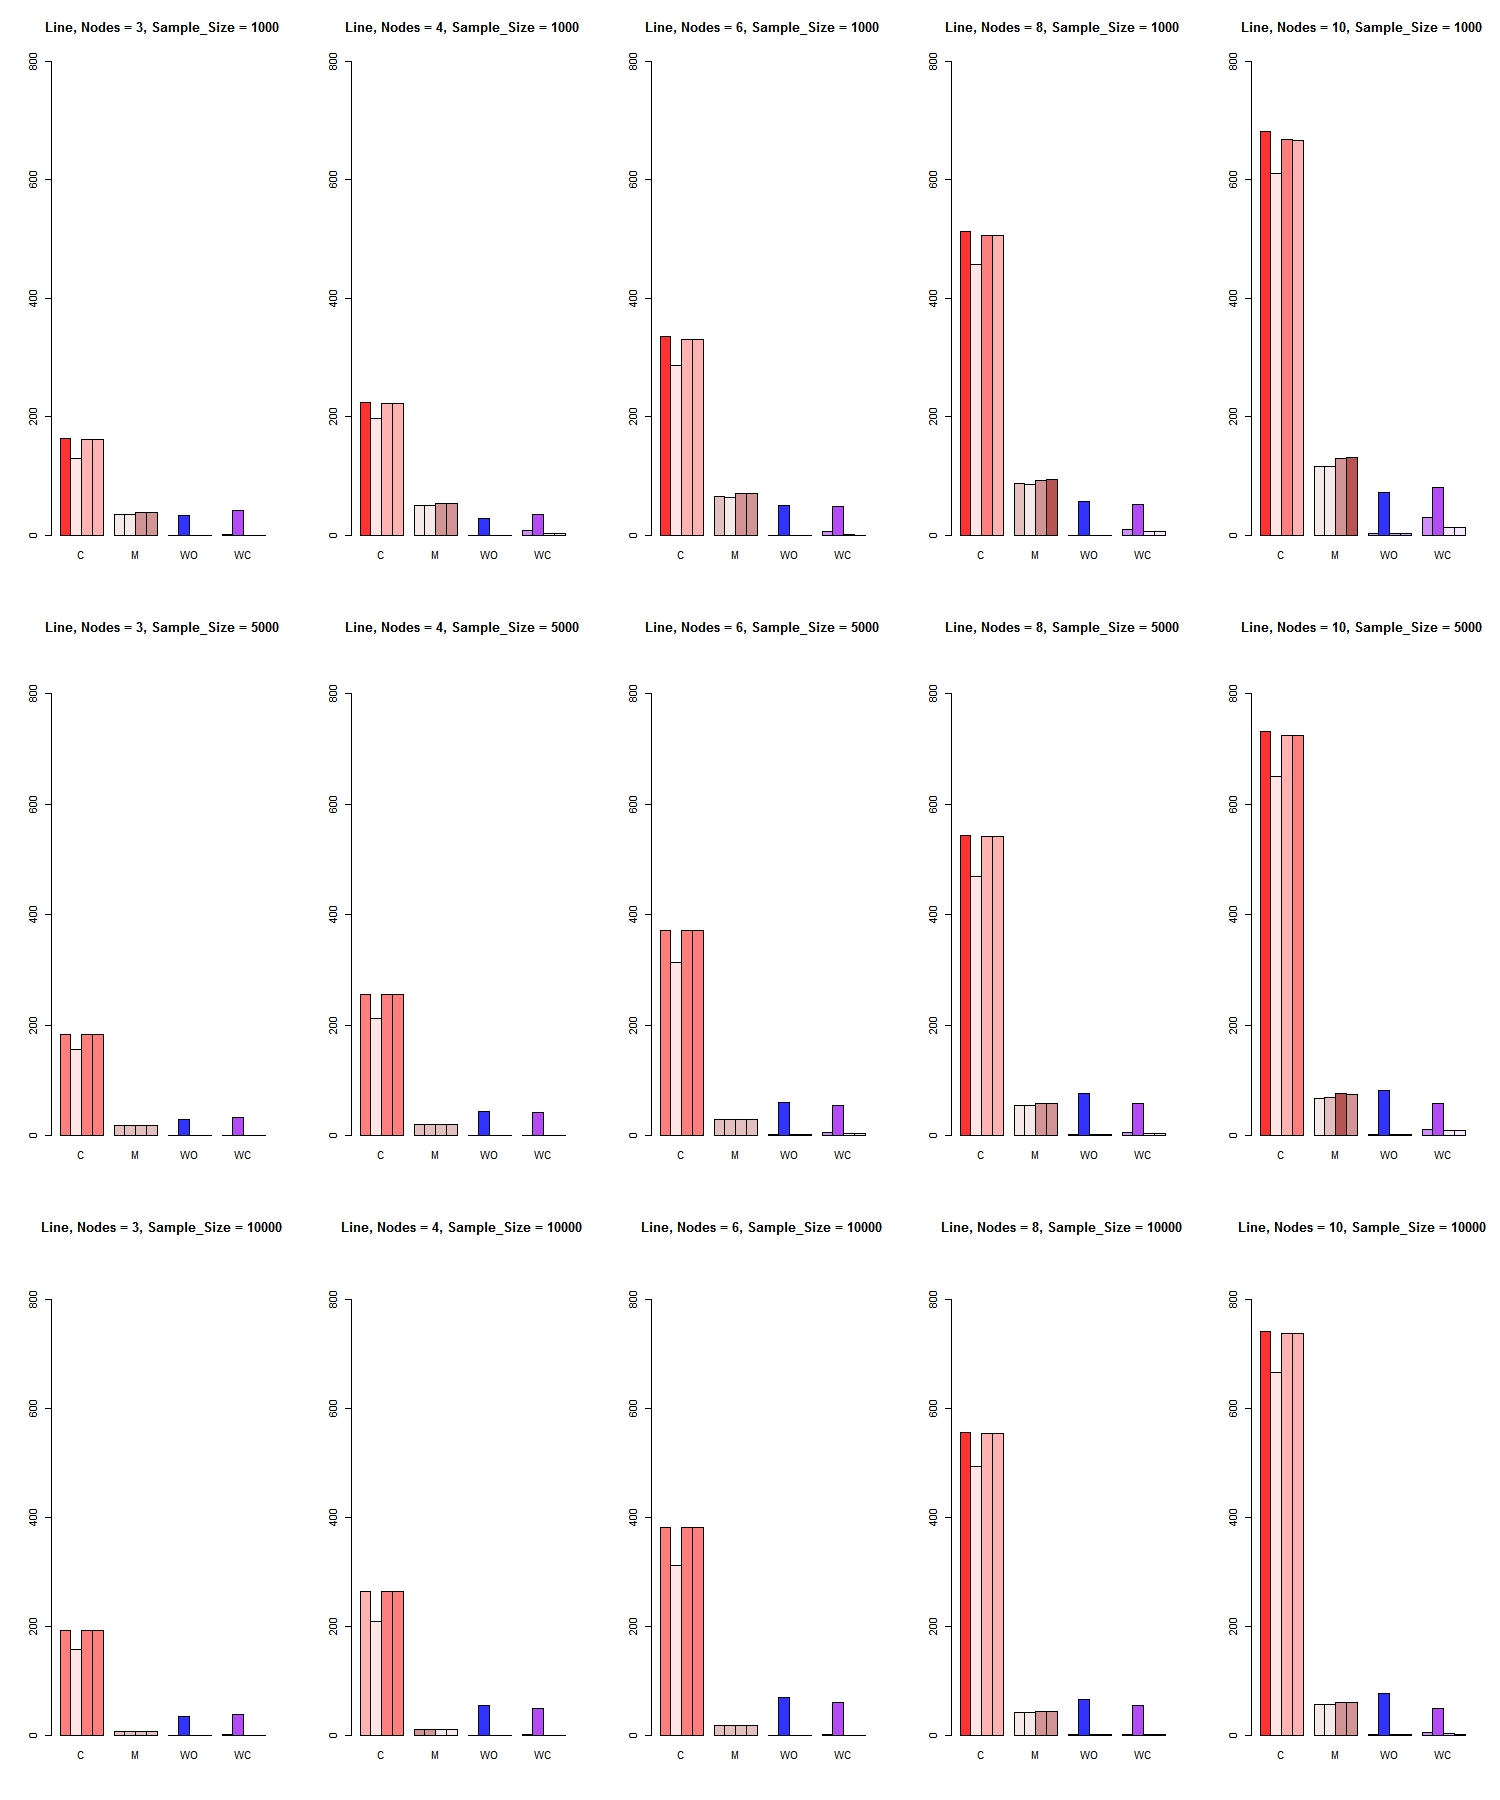
\includegraphics[height=170pt]{images/02_Line_Arcs}
	\end{figure}	
}
\end{frame}



\begin{frame}
\frametitle{Topology에 따른 비교 : Line}
{\scriptsize{}
	\begin{center}
		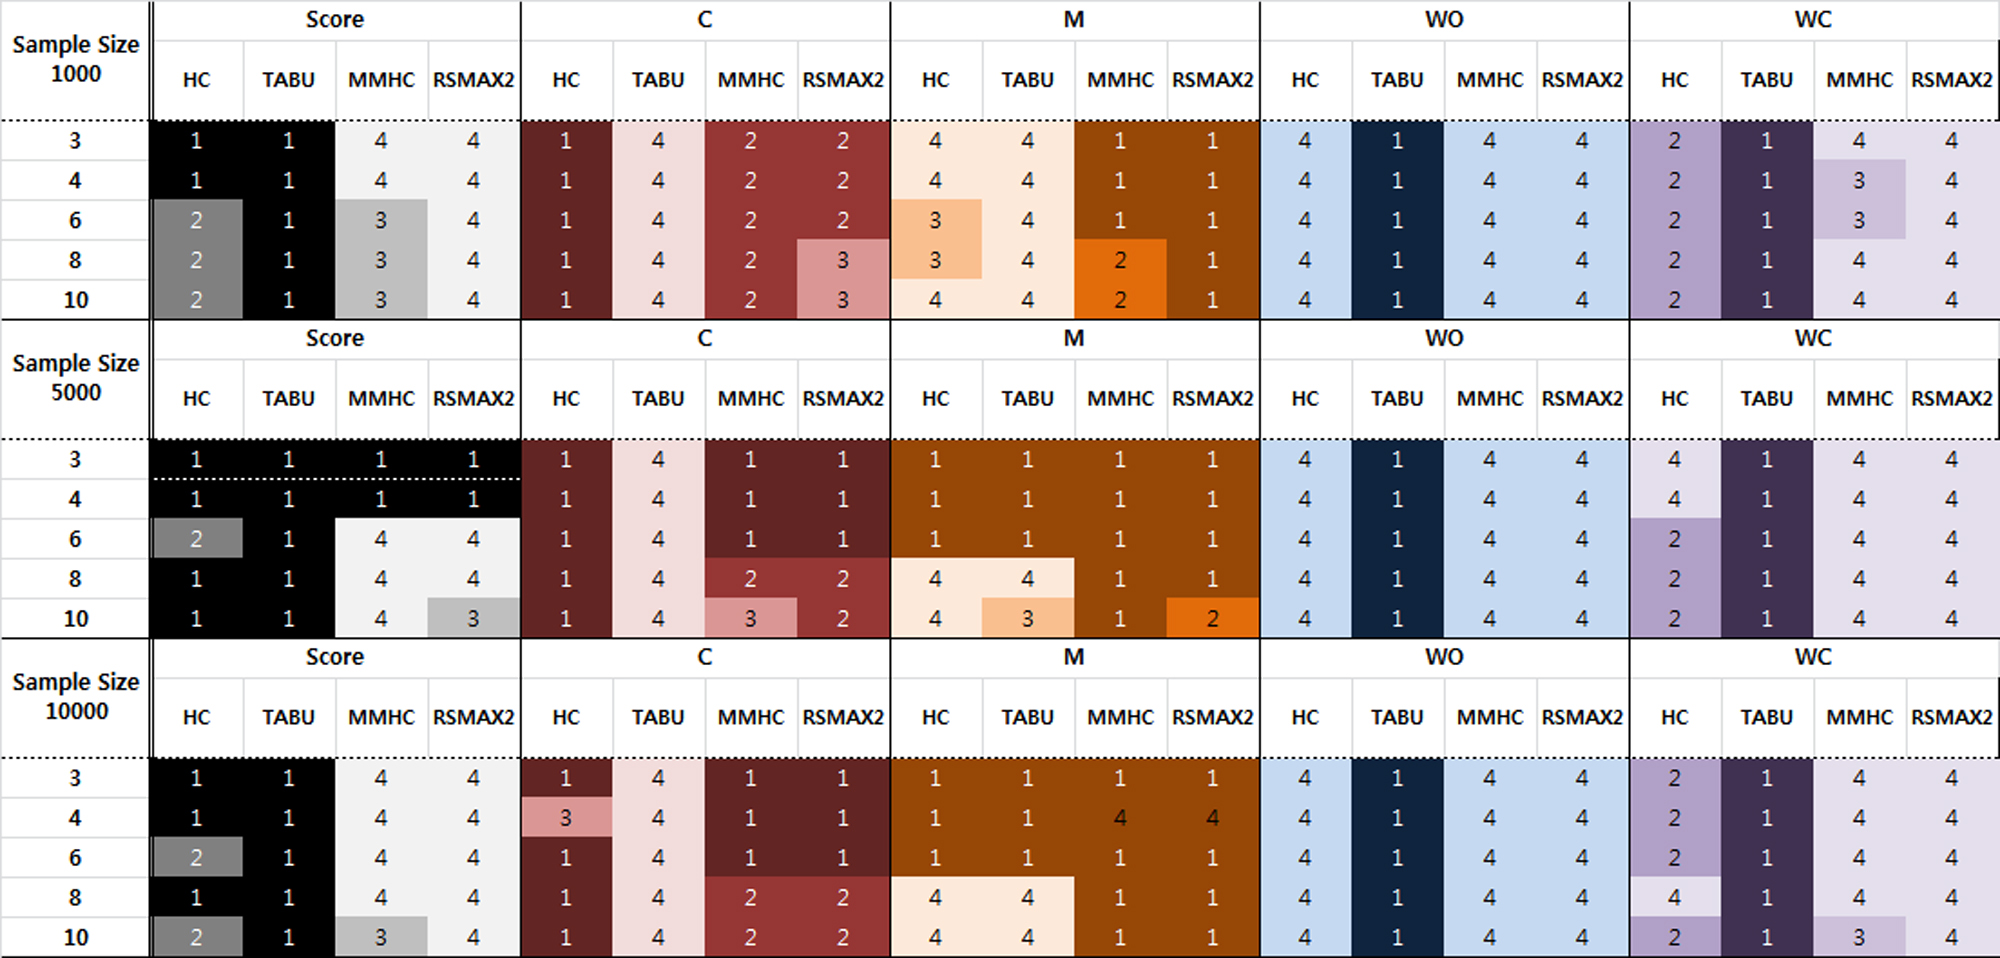
\includegraphics[height=130pt]{images/Result_Line}
	\end{center}
}
\end{frame}



\begin{frame}
\frametitle{Topology에 따른 비교 분석 : Star}
{\scriptsize{}
	\begin{figure}
		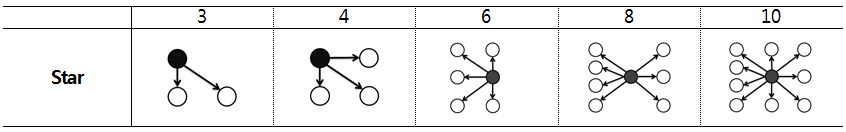
\includegraphics[height=50pt]{images/Topologies_Star}
	\end{figure}	
}
\end{frame}



\begin{frame}
\frametitle{Topology에 따른 비교 : Star (Score)}
{\scriptsize{}
	\begin{figure}
		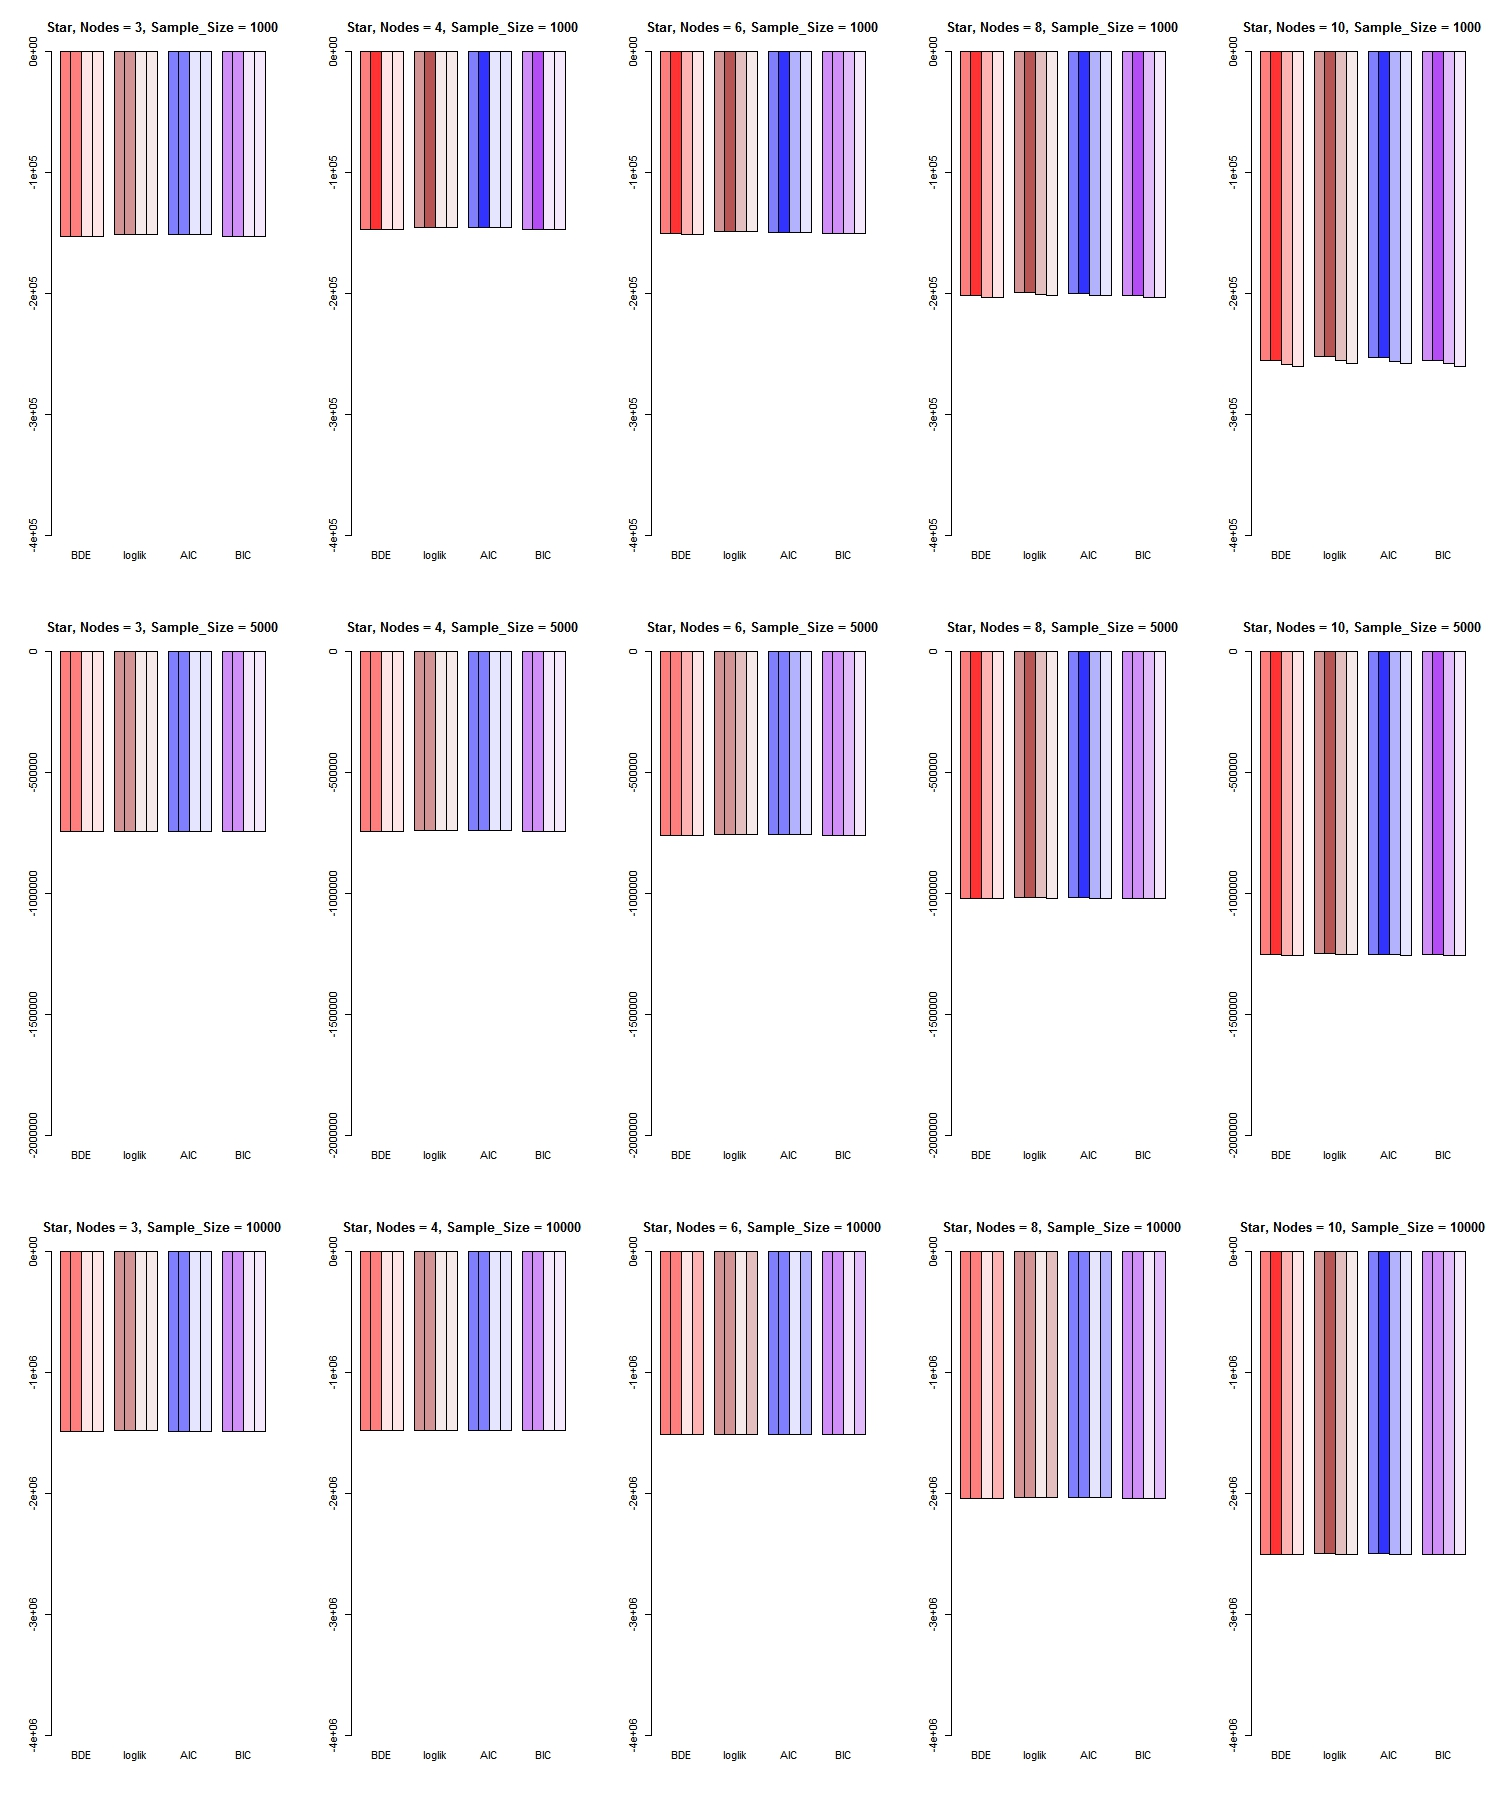
\includegraphics[height=170pt]{images/03_Star_Score}
	\end{figure}	
}
\end{frame}


\begin{frame}
\frametitle{Topology에 따른 비교 : Star (Arcs)}
{\scriptsize{}
	\begin{figure}
		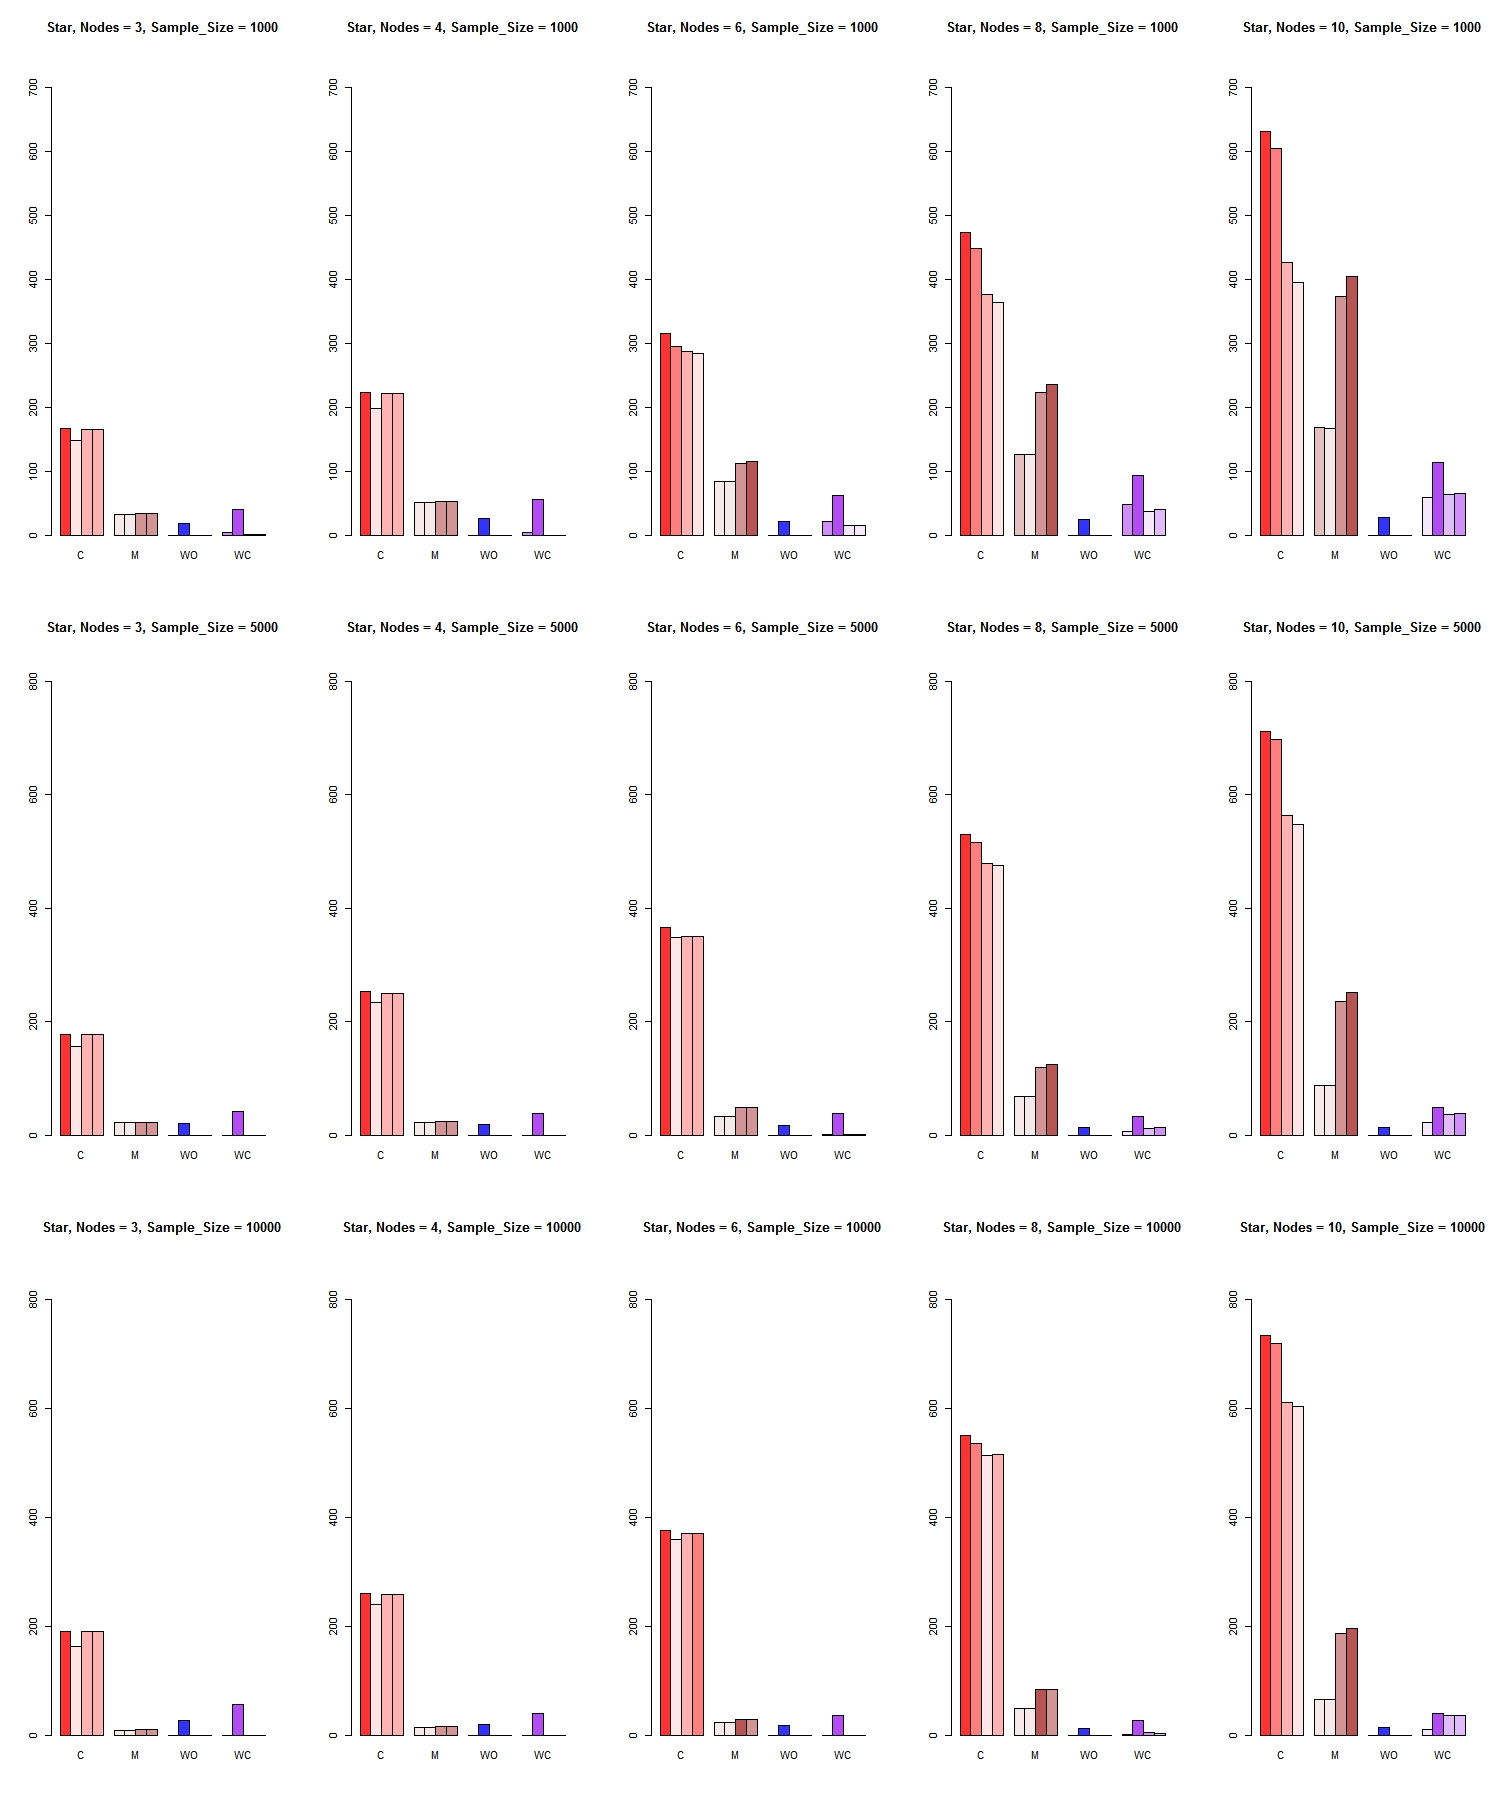
\includegraphics[height=170pt]{images/03_Star_Arcs}
	\end{figure}	
}
\end{frame}



\begin{frame}
\frametitle{Topology에 따른 비교 분석 : Star}
{\scriptsize{}
	\begin{center}
		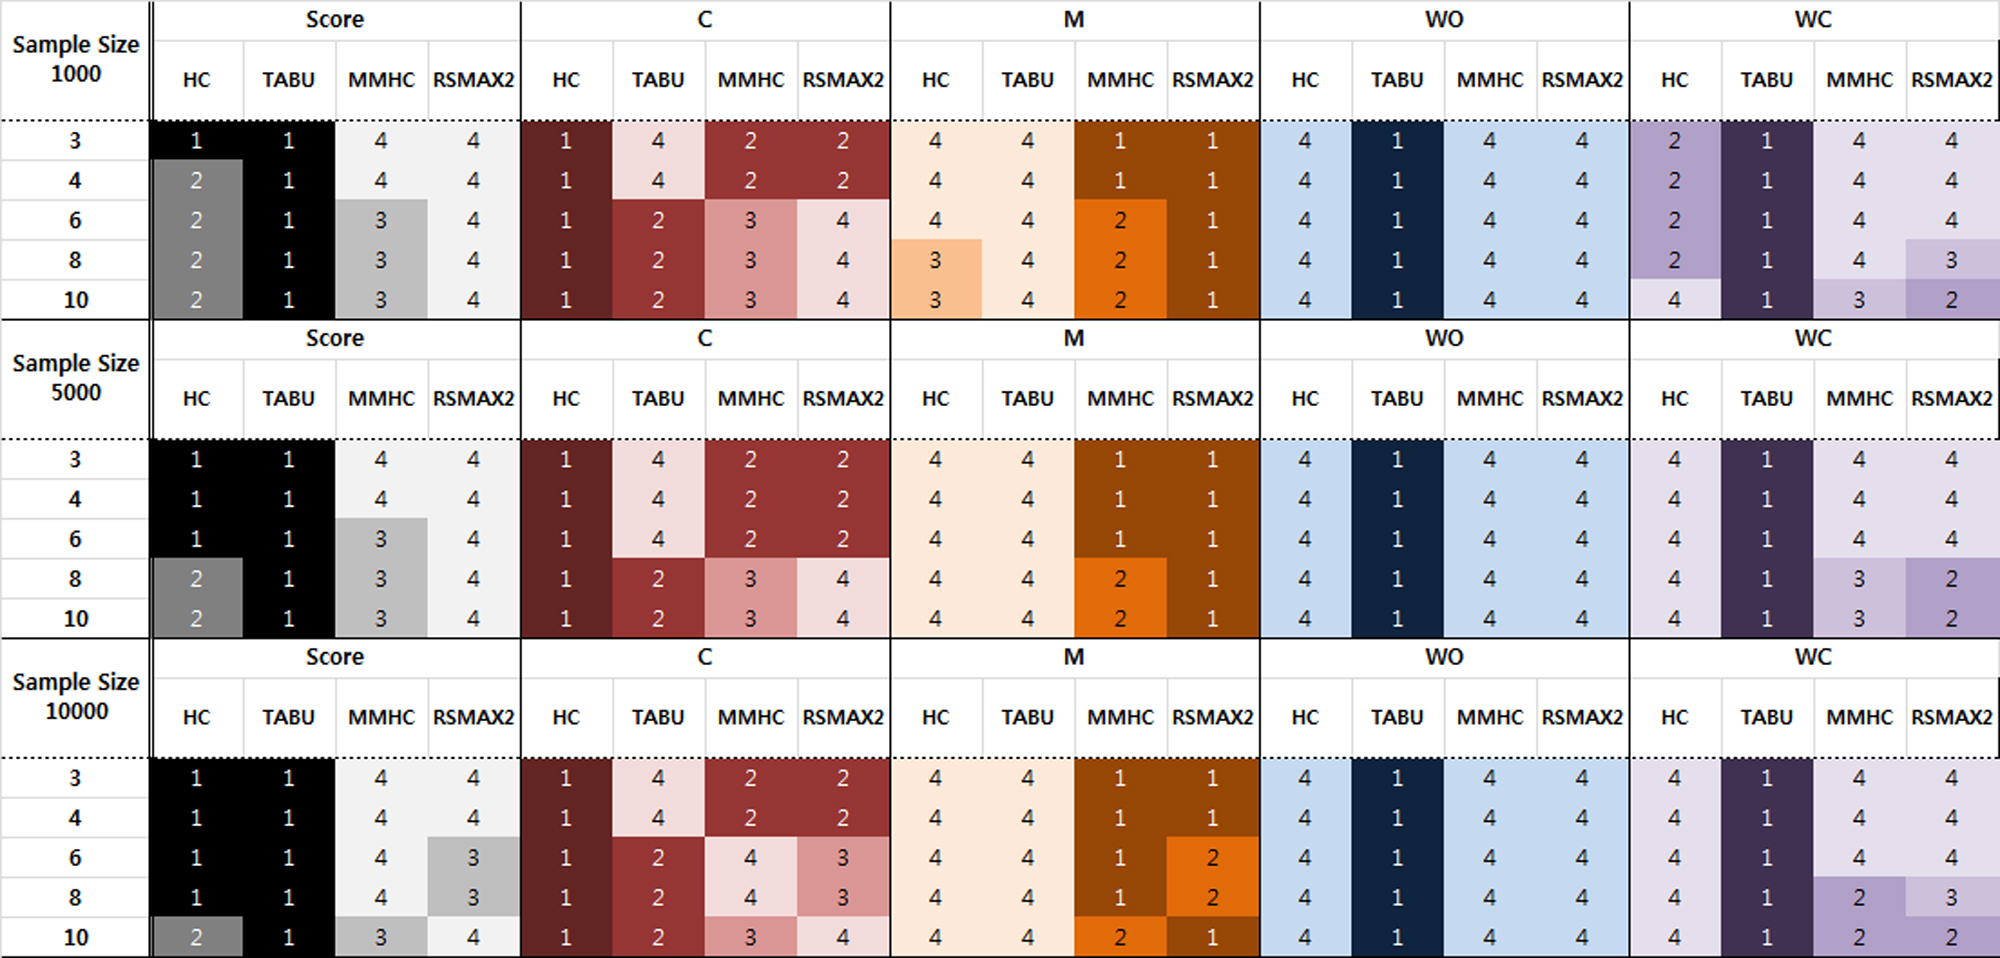
\includegraphics[height=130pt]{images/Result_Star}
	\end{center}
}
\end{frame}



\begin{frame}
\frametitle{Topology에 따른 비교 분석 : PseudoLoop}
{\scriptsize{}
	\begin{figure}
		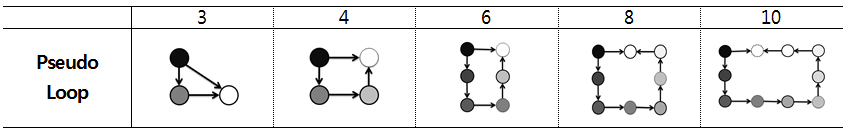
\includegraphics[height=50pt]{images/Topologies_PseudoLoop}
	\end{figure}	
}
\end{frame}



\begin{frame}
\frametitle{Topology에 따른 비교 분석 : PseudoLoop (Score)}
{\scriptsize{}
	\begin{figure}
		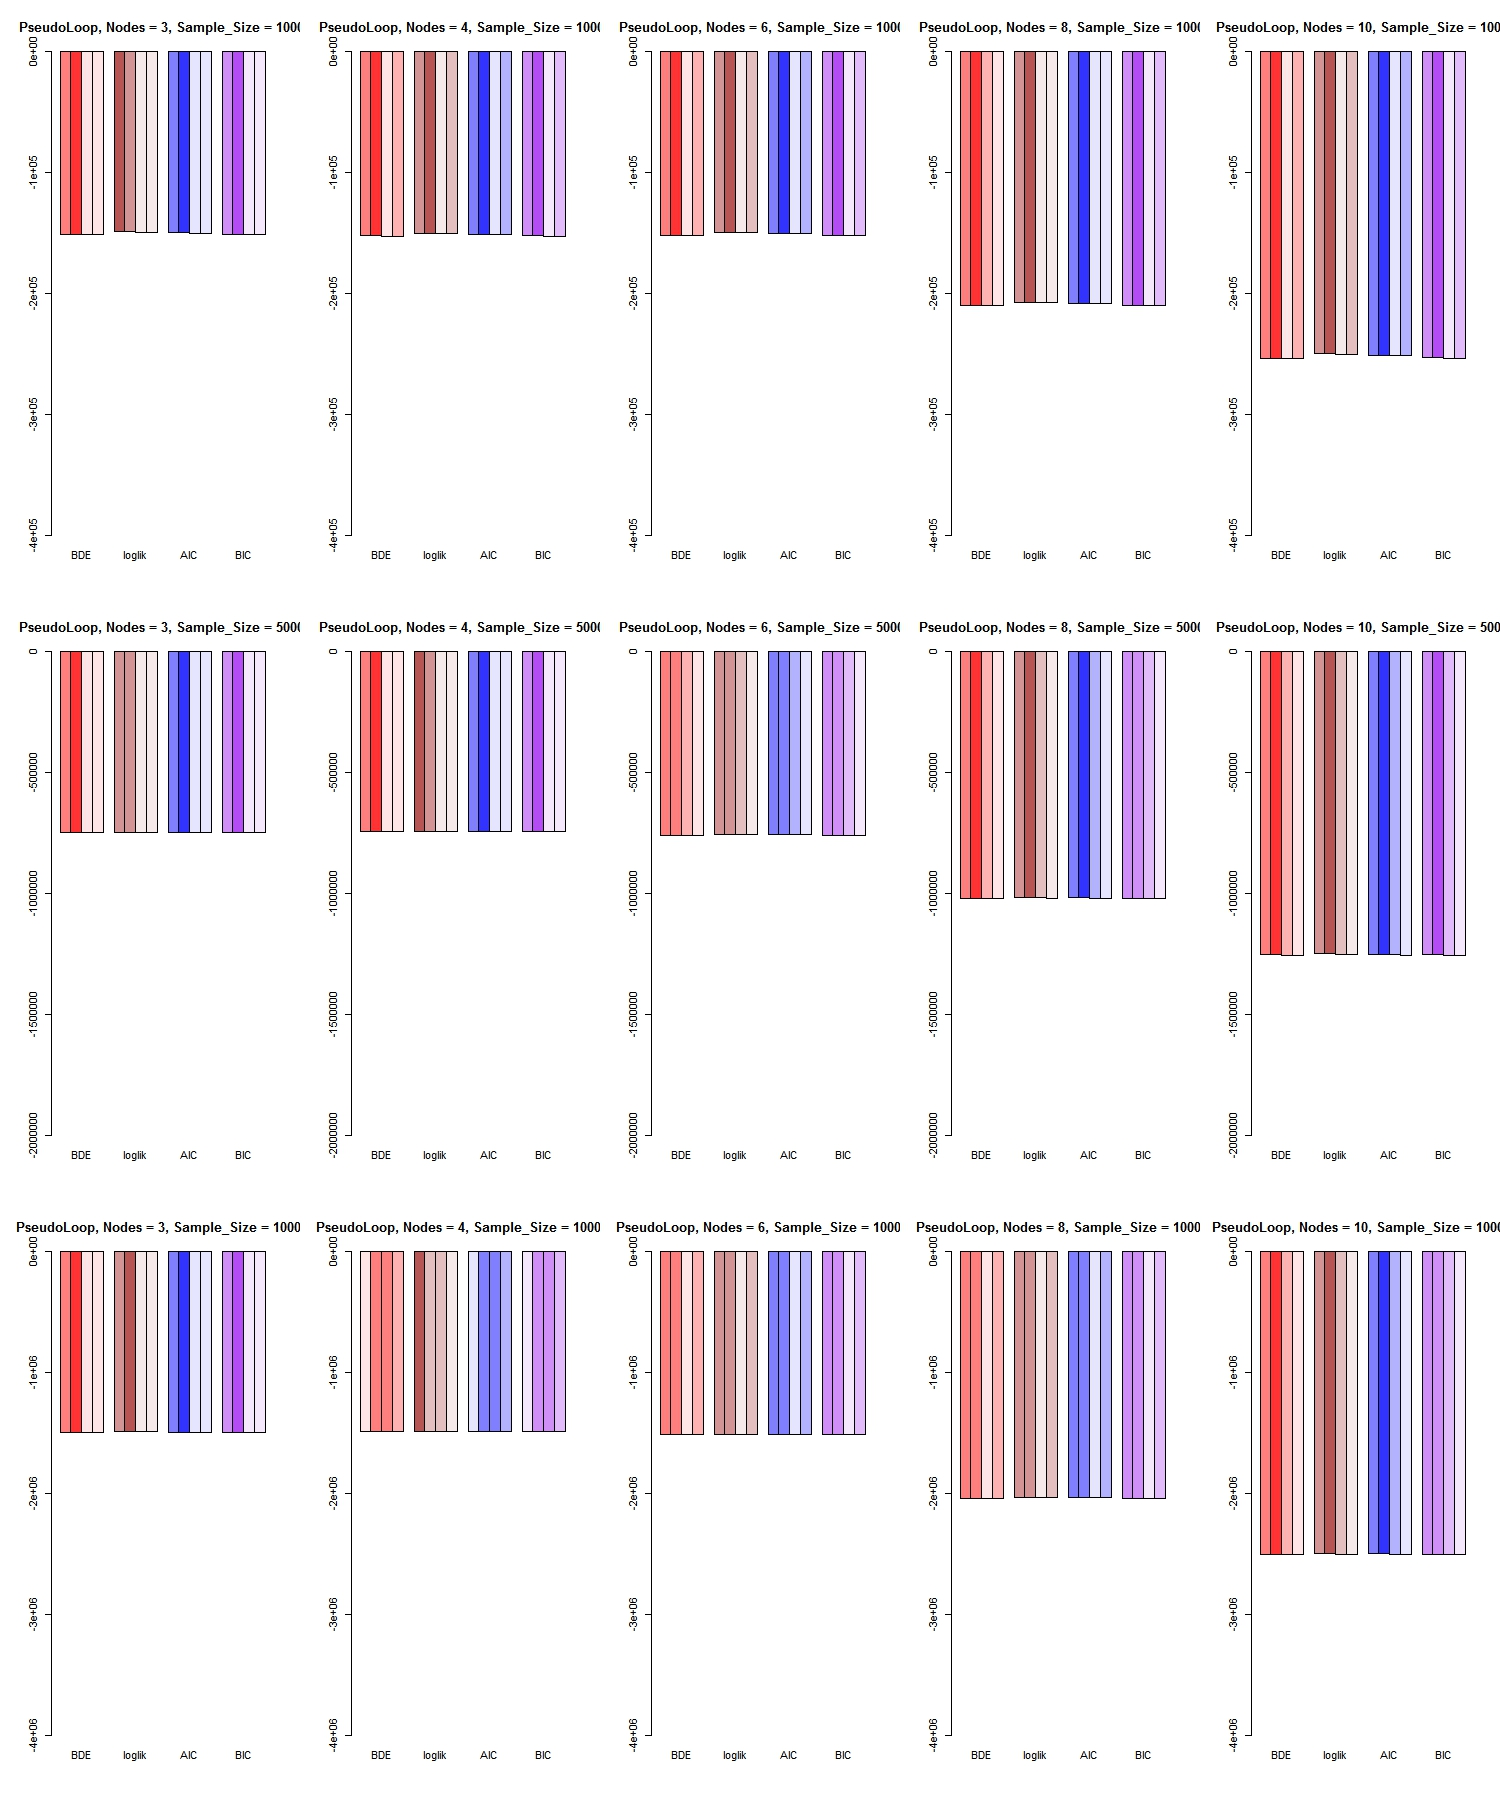
\includegraphics[height=170pt]{images/04_PseudoLoop_Score}
	\end{figure}	
}
\end{frame}


\begin{frame}
\frametitle{Topology에 따른 비교 분석 : PseudoLoop (Arc)}
{\scriptsize{}
	\begin{figure}
		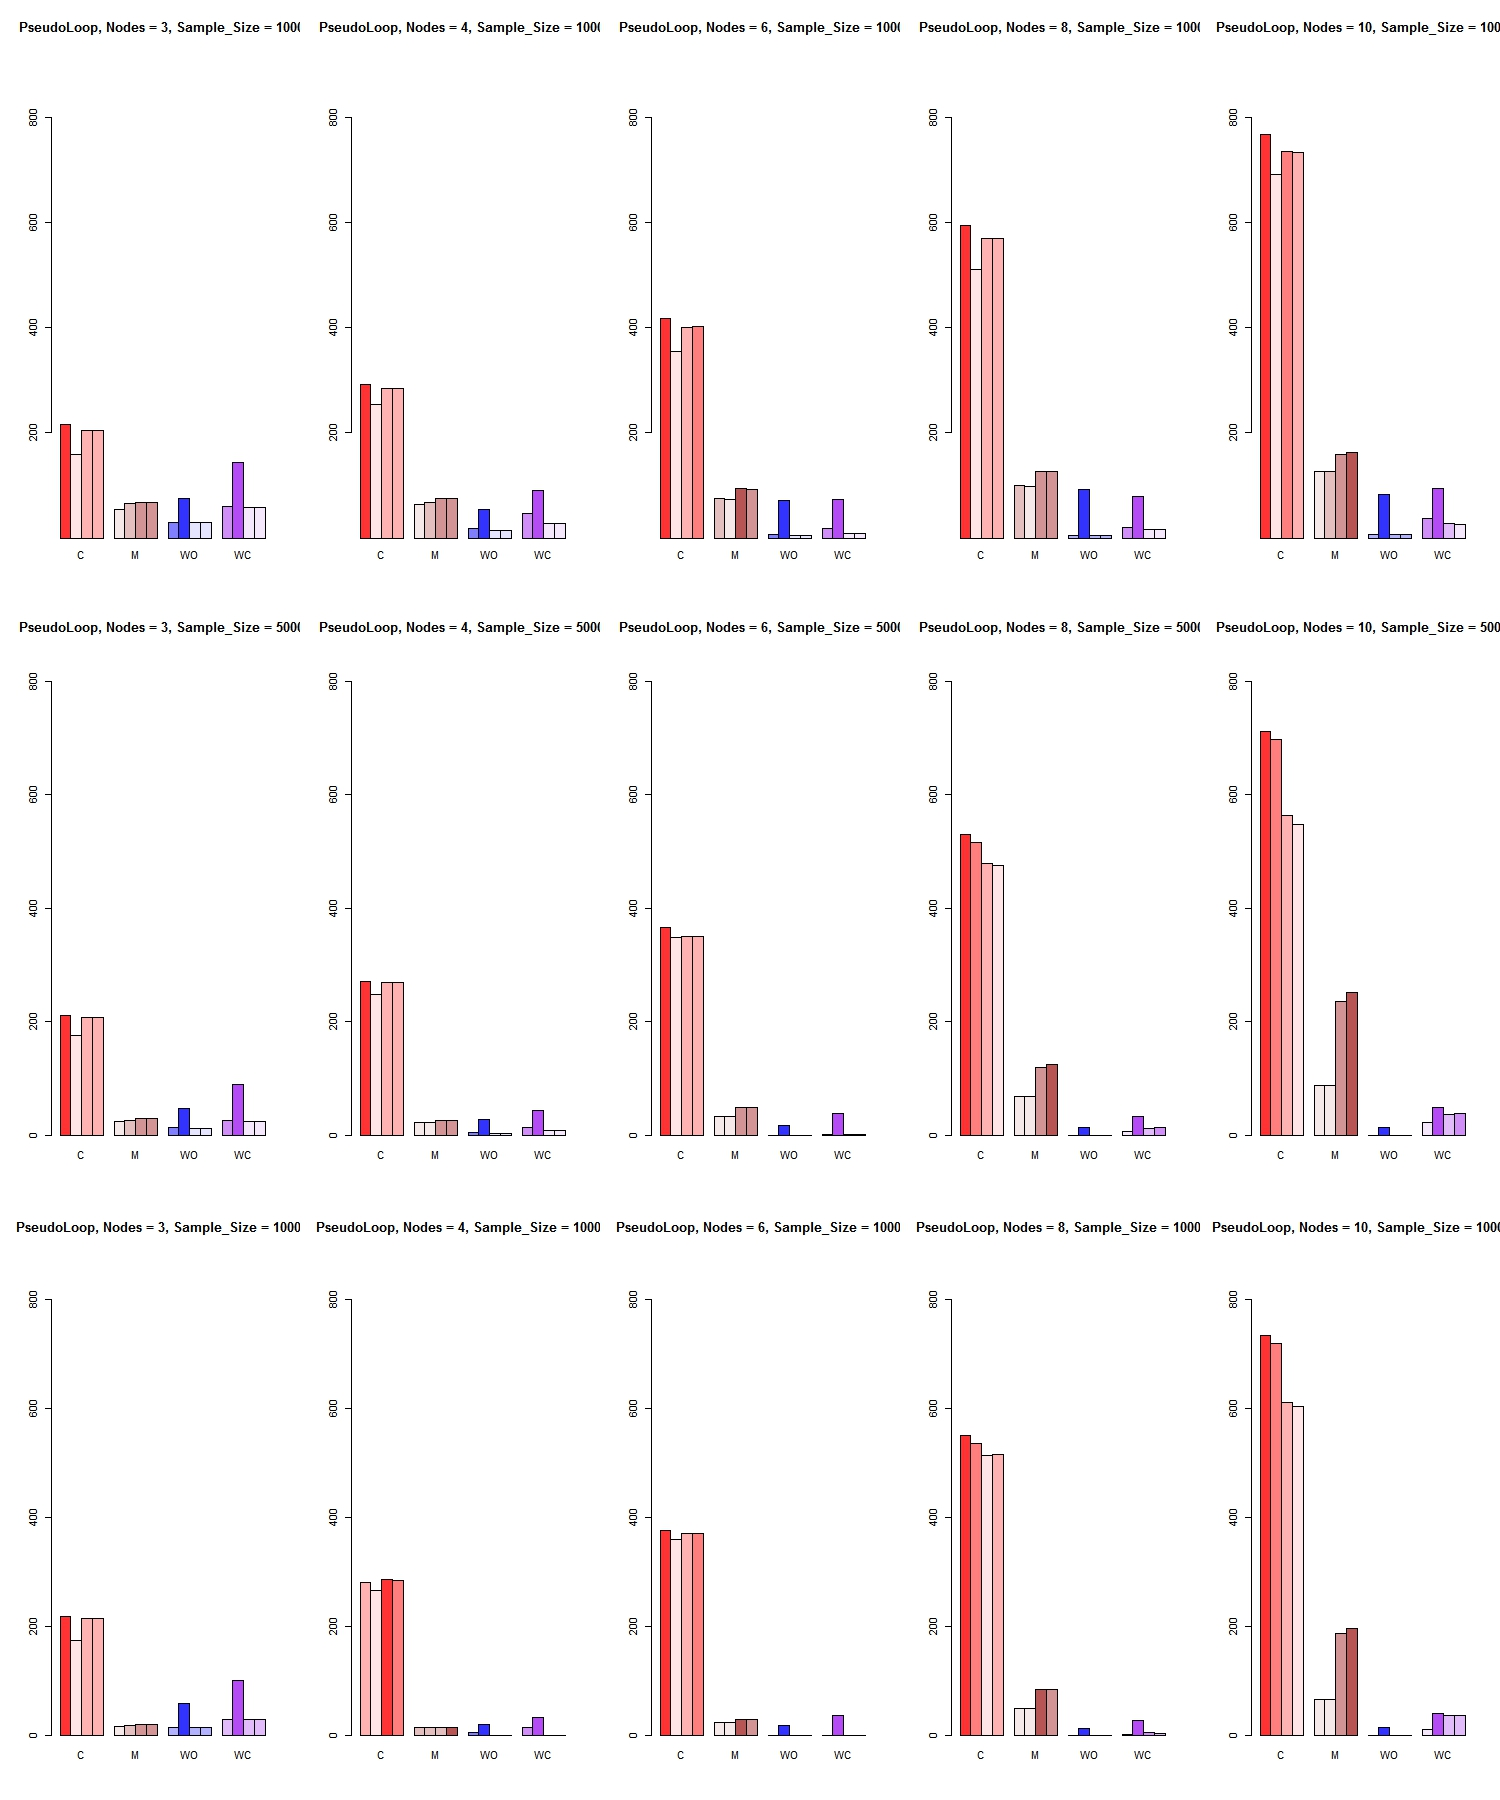
\includegraphics[height=170pt]{images/04_PseudoLoop_Arcs}
	\end{figure}	
}
\end{frame}


\begin{frame}
\frametitle{Topology에 따른 비교 분석 : PseudoLoop}
{\scriptsize{}
	\begin{center}
		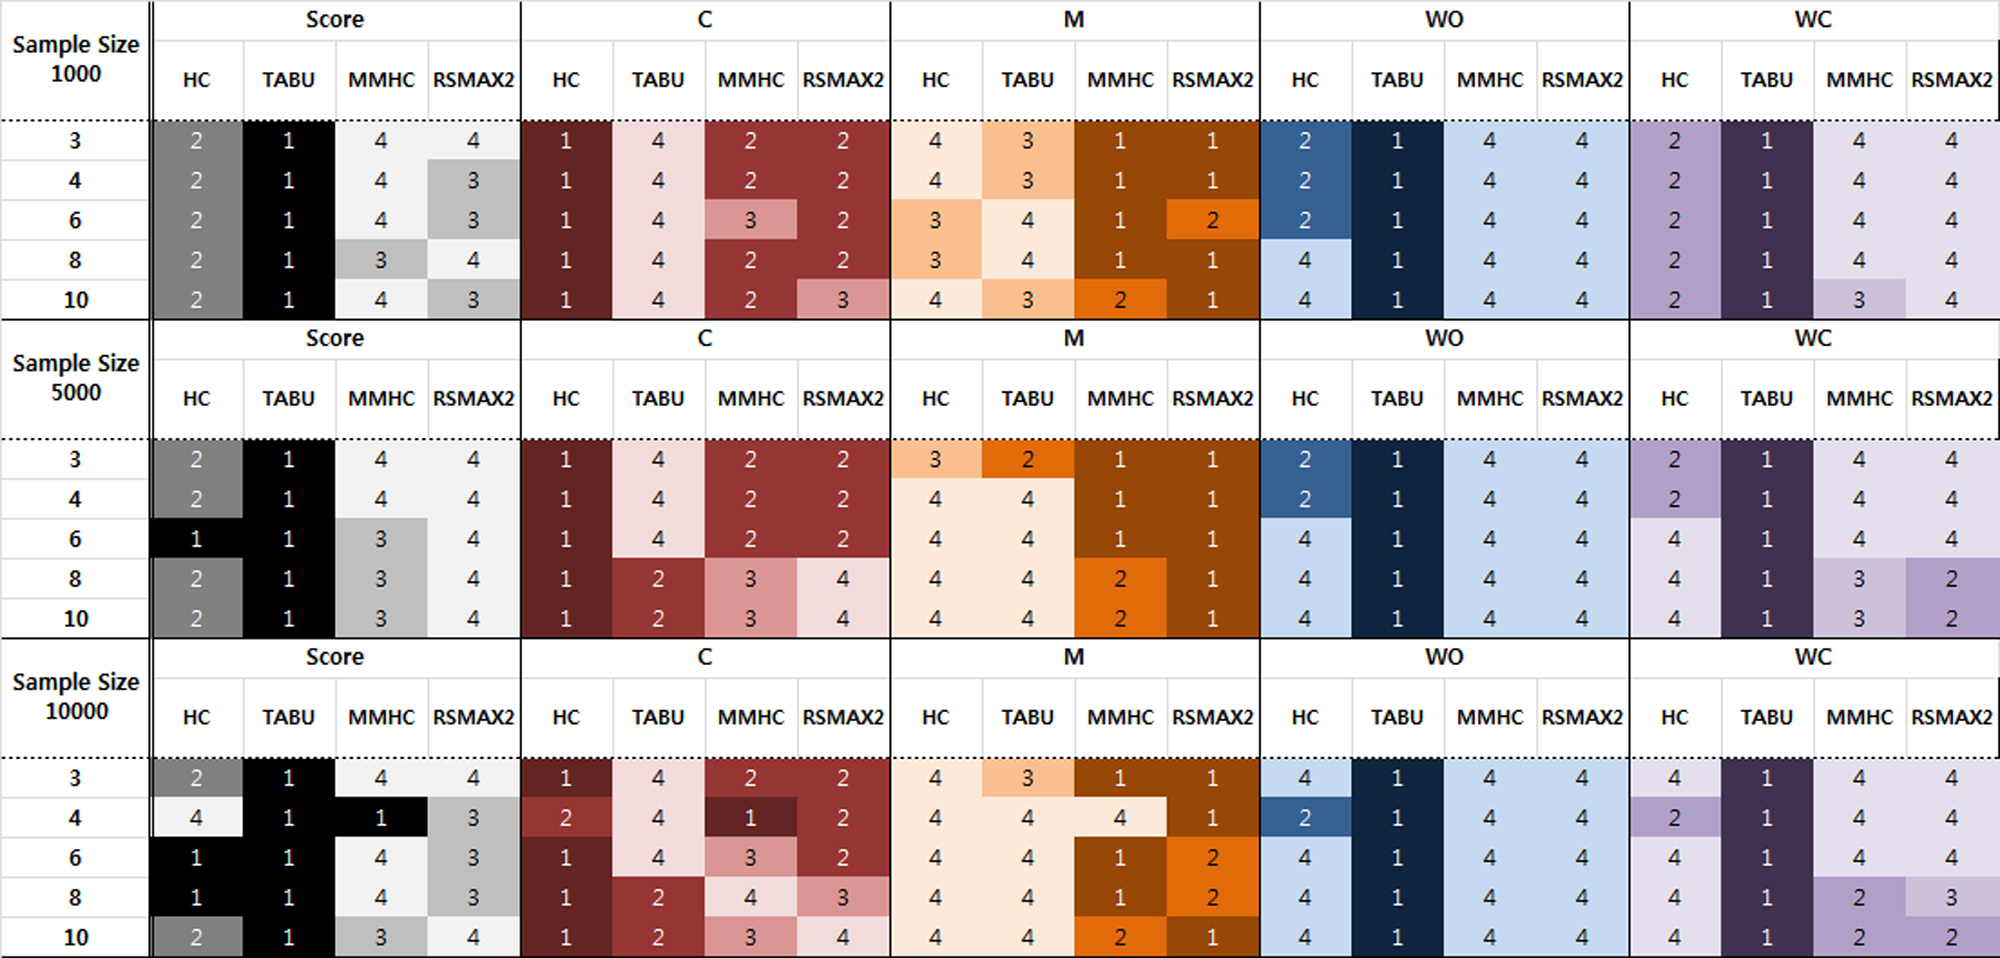
\includegraphics[height=130pt]{images/Result_PseudoLoop}
	\end{center}
}
\end{frame}




\begin{frame}
\frametitle{Topology에 따른 비교 분석 : Diamond}
{\scriptsize{}
	\begin{figure}
		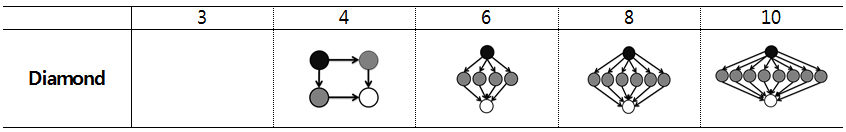
\includegraphics[height=50pt]{images/Topologies_Diamond}
	\end{figure}	
}
\end{frame}



\begin{frame}
\frametitle{Topology에 따른 비교 분석 : Diamond (Score)}
{\scriptsize{}
	\begin{figure}
		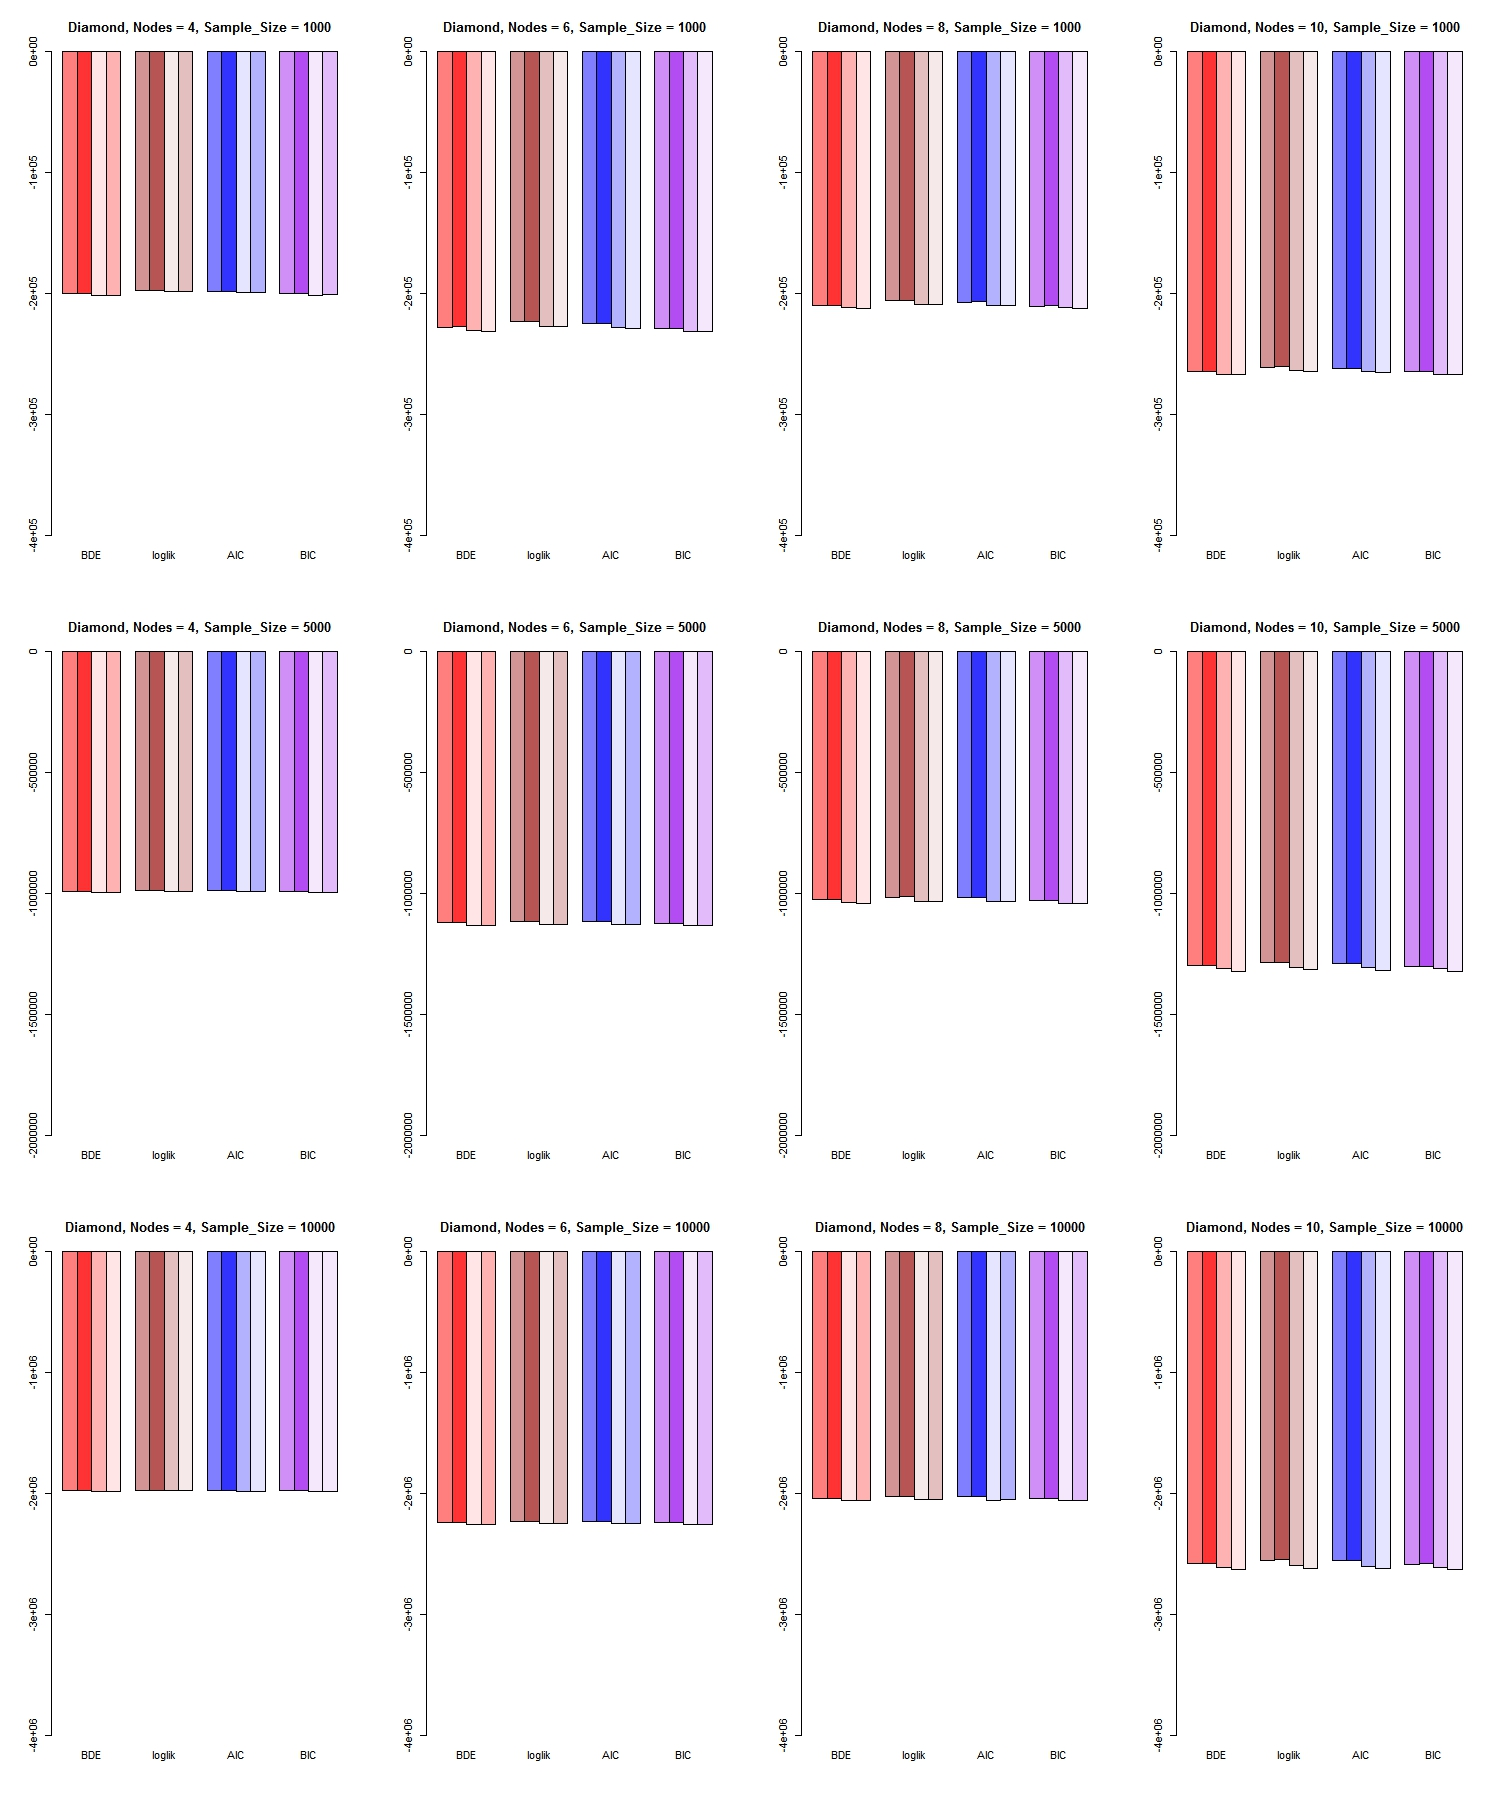
\includegraphics[height=170pt]{images/05_Diamond_Score}
	\end{figure}	
}
\end{frame}


\begin{frame}
\frametitle{Topology에 따른 비교 분석 : Diamond (Arc)}
{\scriptsize{}
	\begin{figure}
		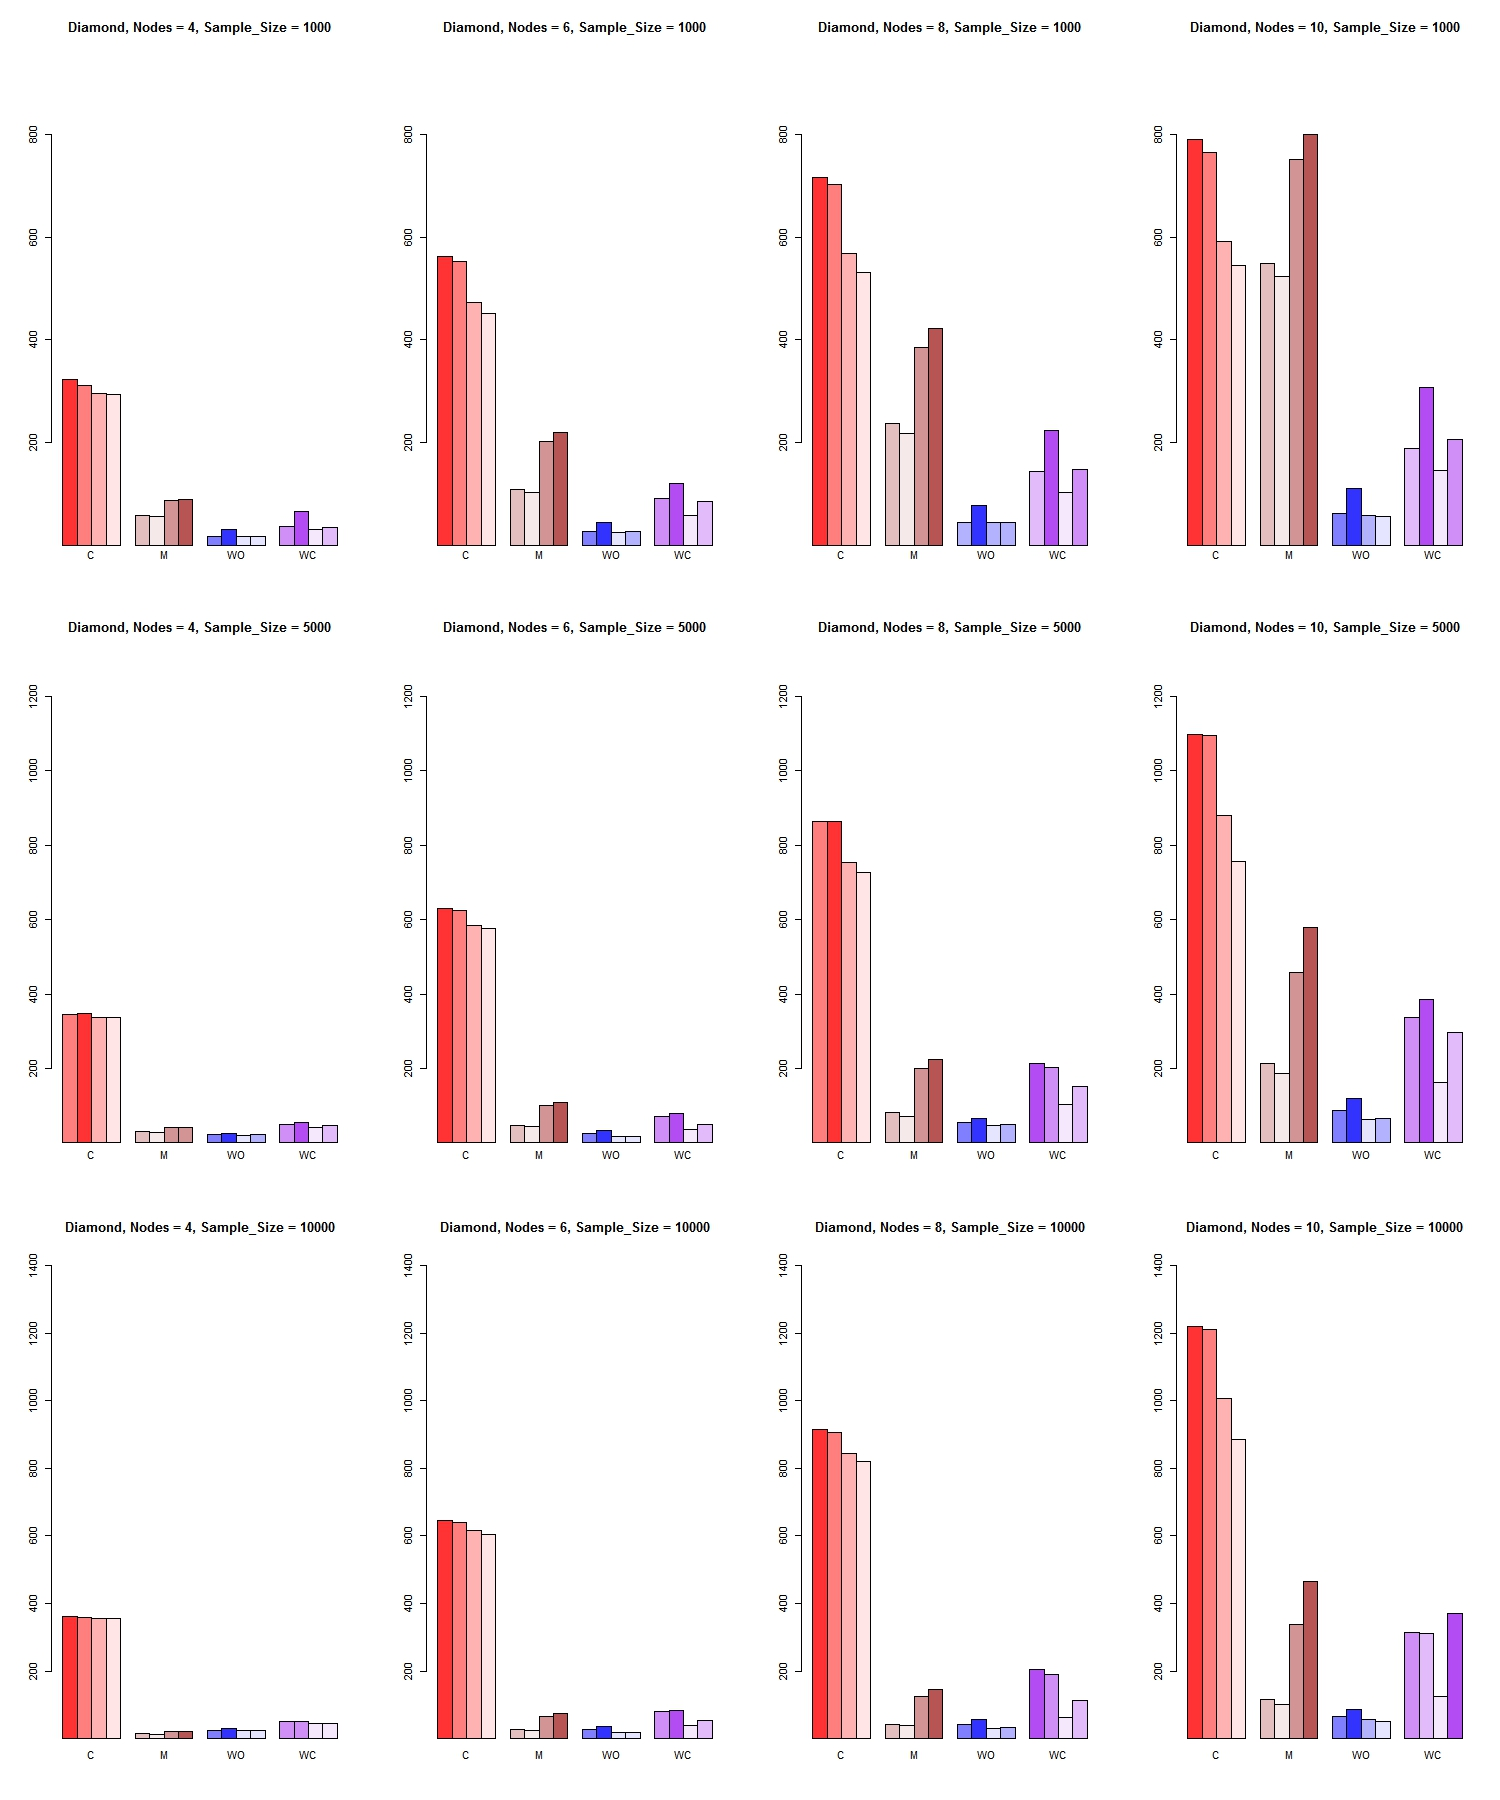
\includegraphics[height=170pt]{images/05_Diamond_Arcs}
	\end{figure}	
}
\end{frame}


\begin{frame}
\frametitle{Topology에 따른 비교 분석 : Diamond}
{\scriptsize{}
	\begin{center}
		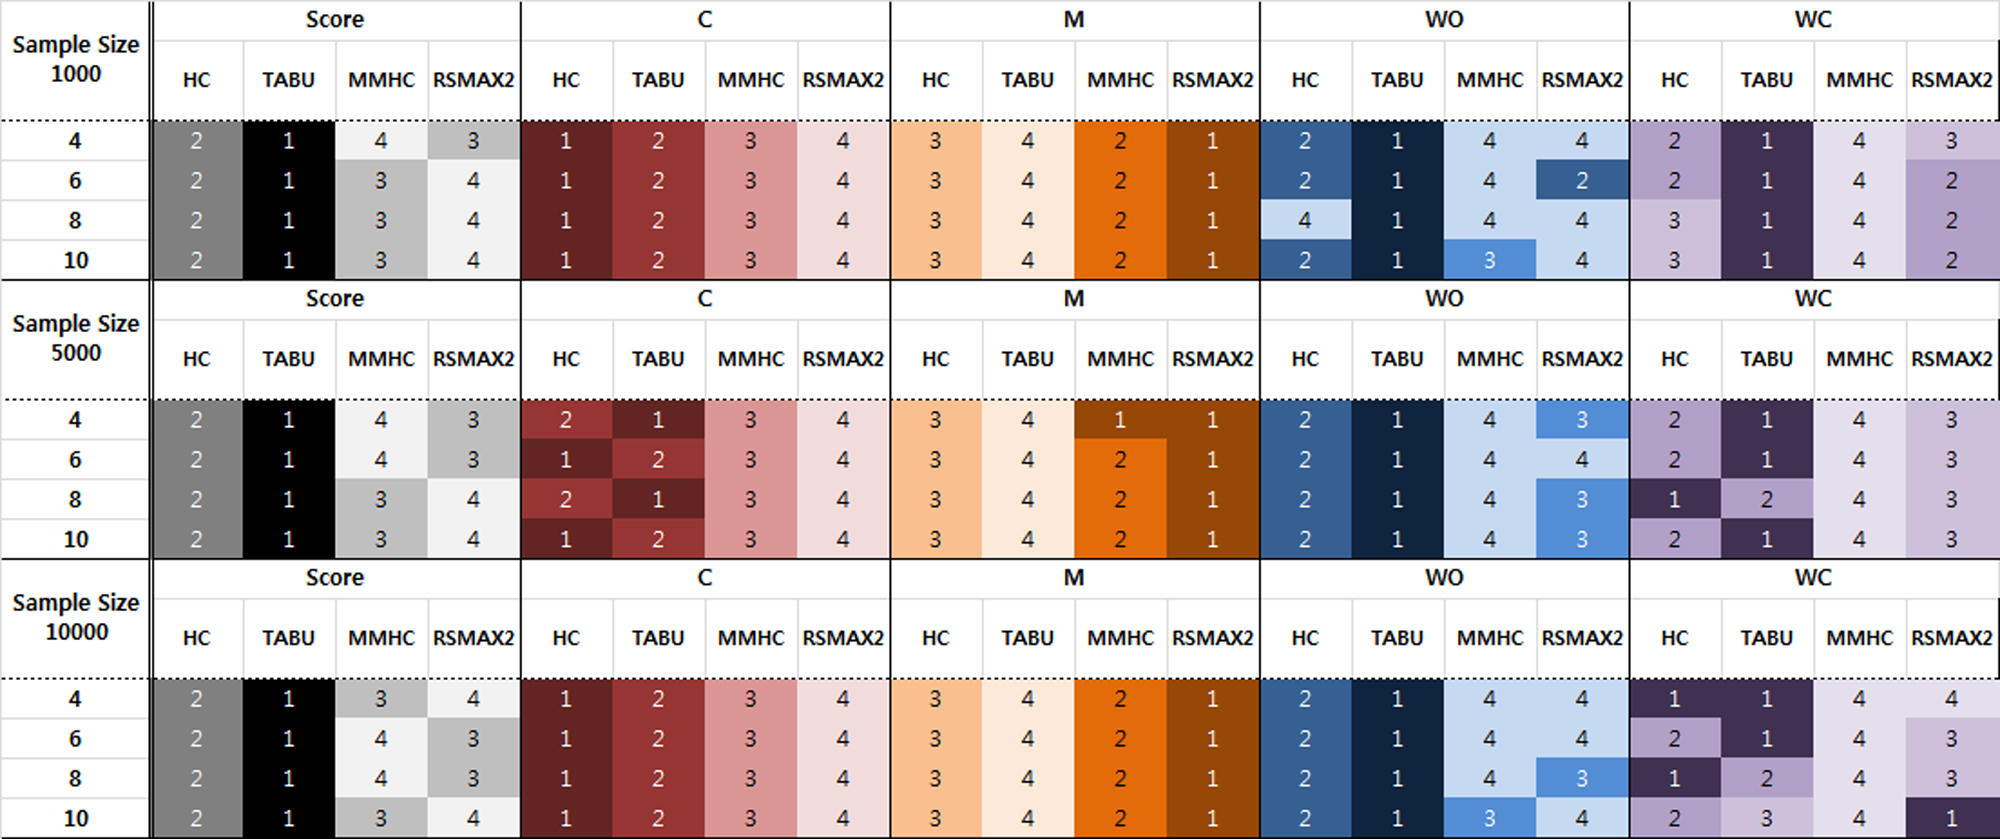
\includegraphics[height=130pt]{images/Result_Diamond}
	\end{center}
}
\end{frame}


\begin{frame}
\frametitle{Topology에 따른 비교 분석 : Rhombus}
{\scriptsize{}
	\begin{figure}
		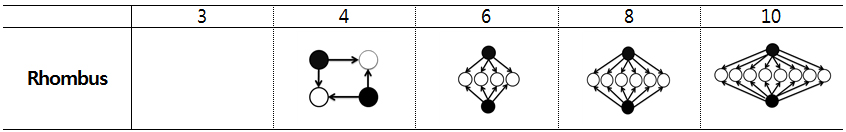
\includegraphics[height=50pt]{images/Topologies_Rhombus}
	\end{figure}	
}
\end{frame}



\begin{frame}
\frametitle{Topology에 따른 비교 분석 : Rhombus (Score)}
{\scriptsize{}
	\begin{figure}
		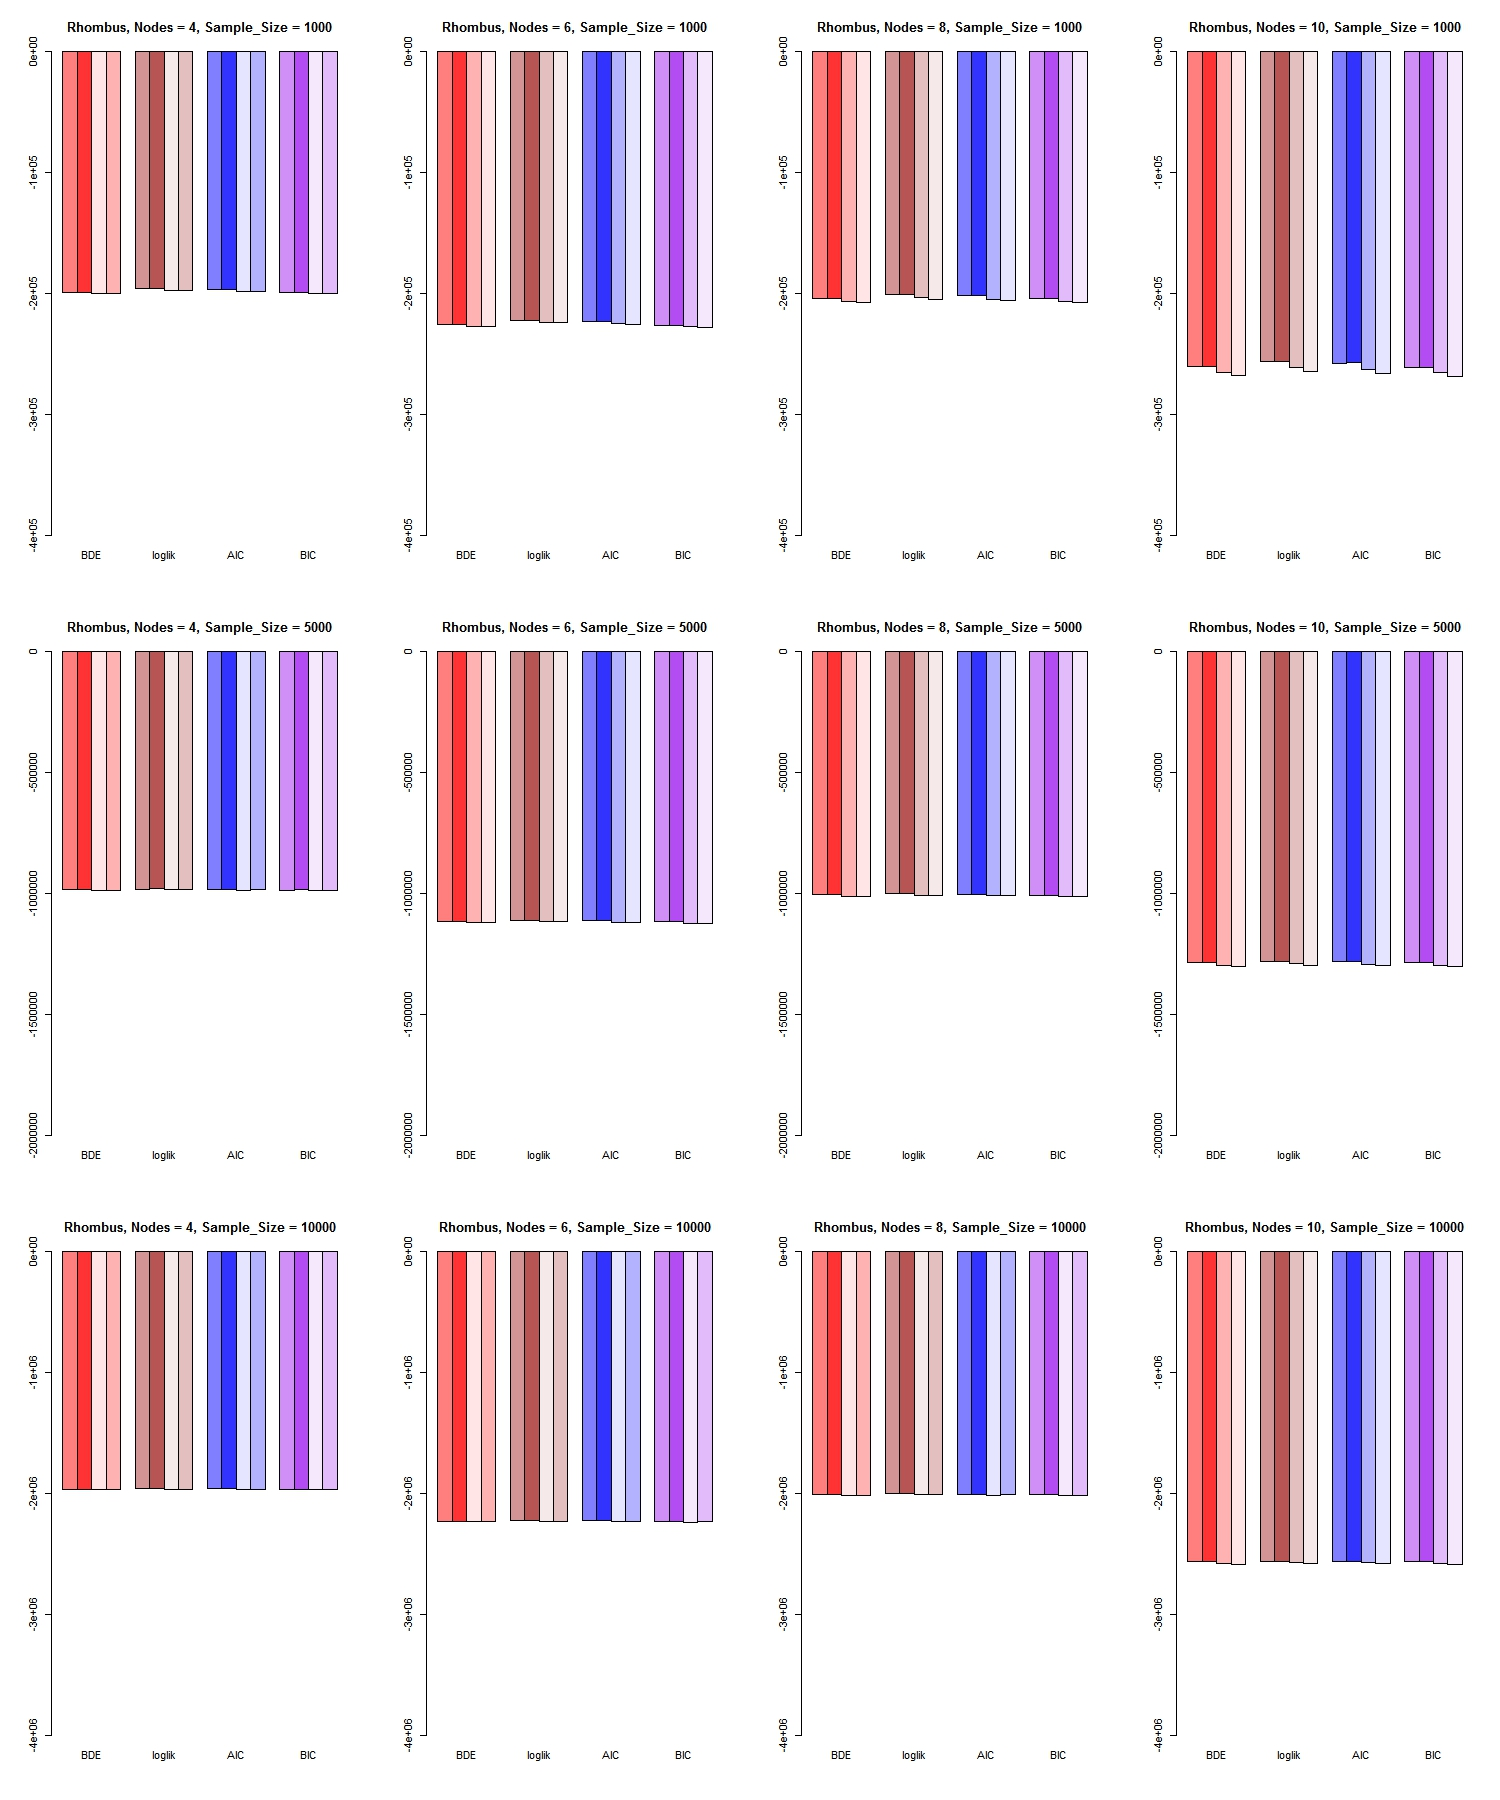
\includegraphics[height=170pt]{images/06_Rhombus_Score}
	\end{figure}	
}
\end{frame}


\begin{frame}
\frametitle{Topology에 따른 비교 분석 : Rhombus (Arc)}
{\scriptsize{}
	\begin{figure}
		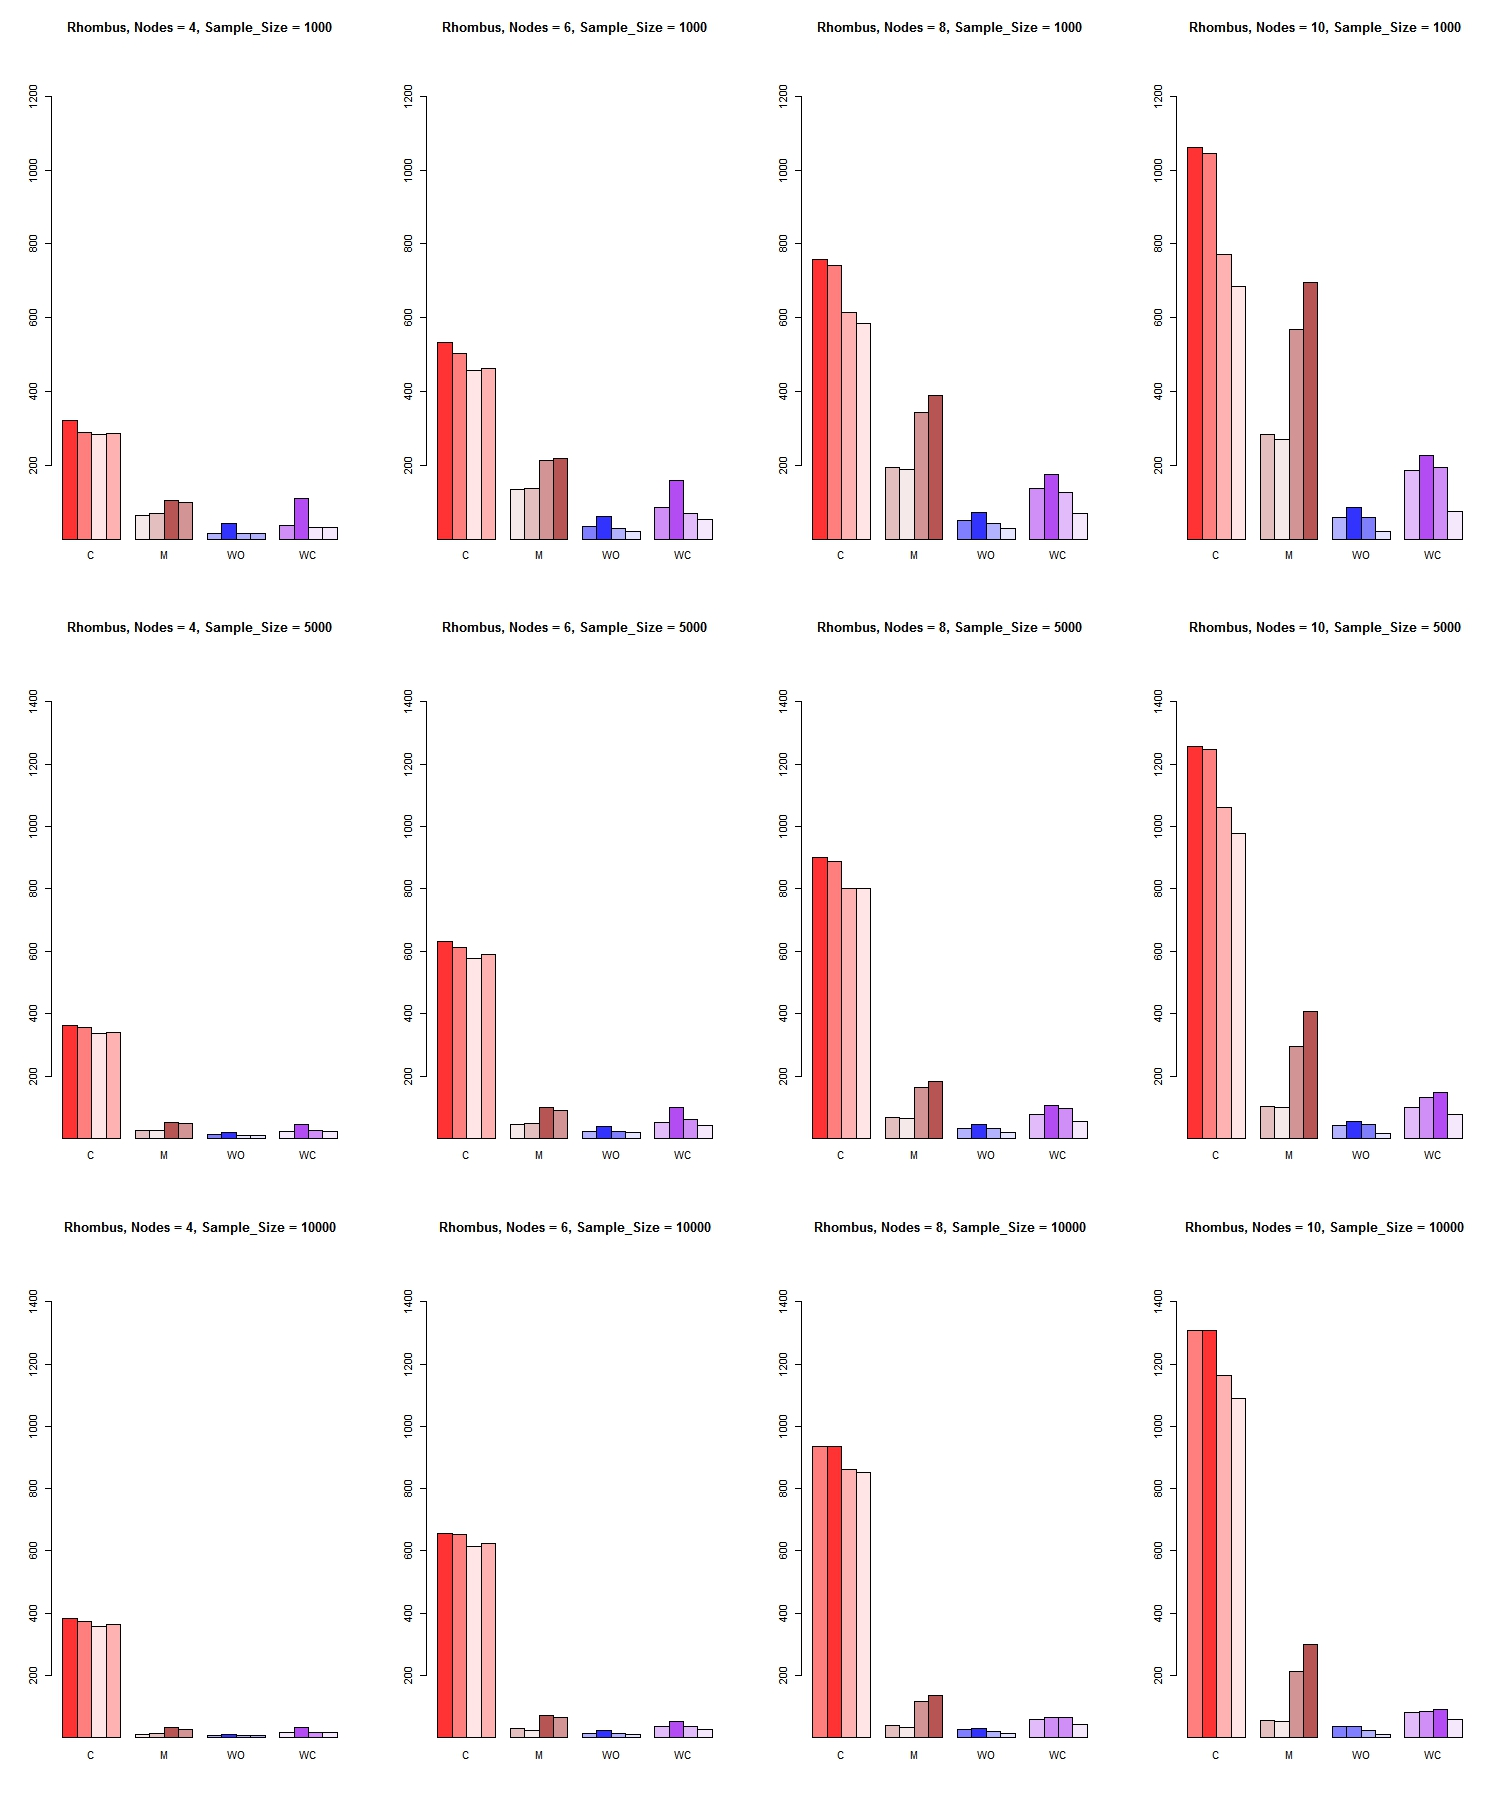
\includegraphics[height=170pt]{images/06_Rhombus_Arcs}
	\end{figure}	
}
\end{frame}



\begin{frame}
\frametitle{Topology에 따른 비교 분석 : Rhombus}
{\scriptsize{}
	\begin{center}
		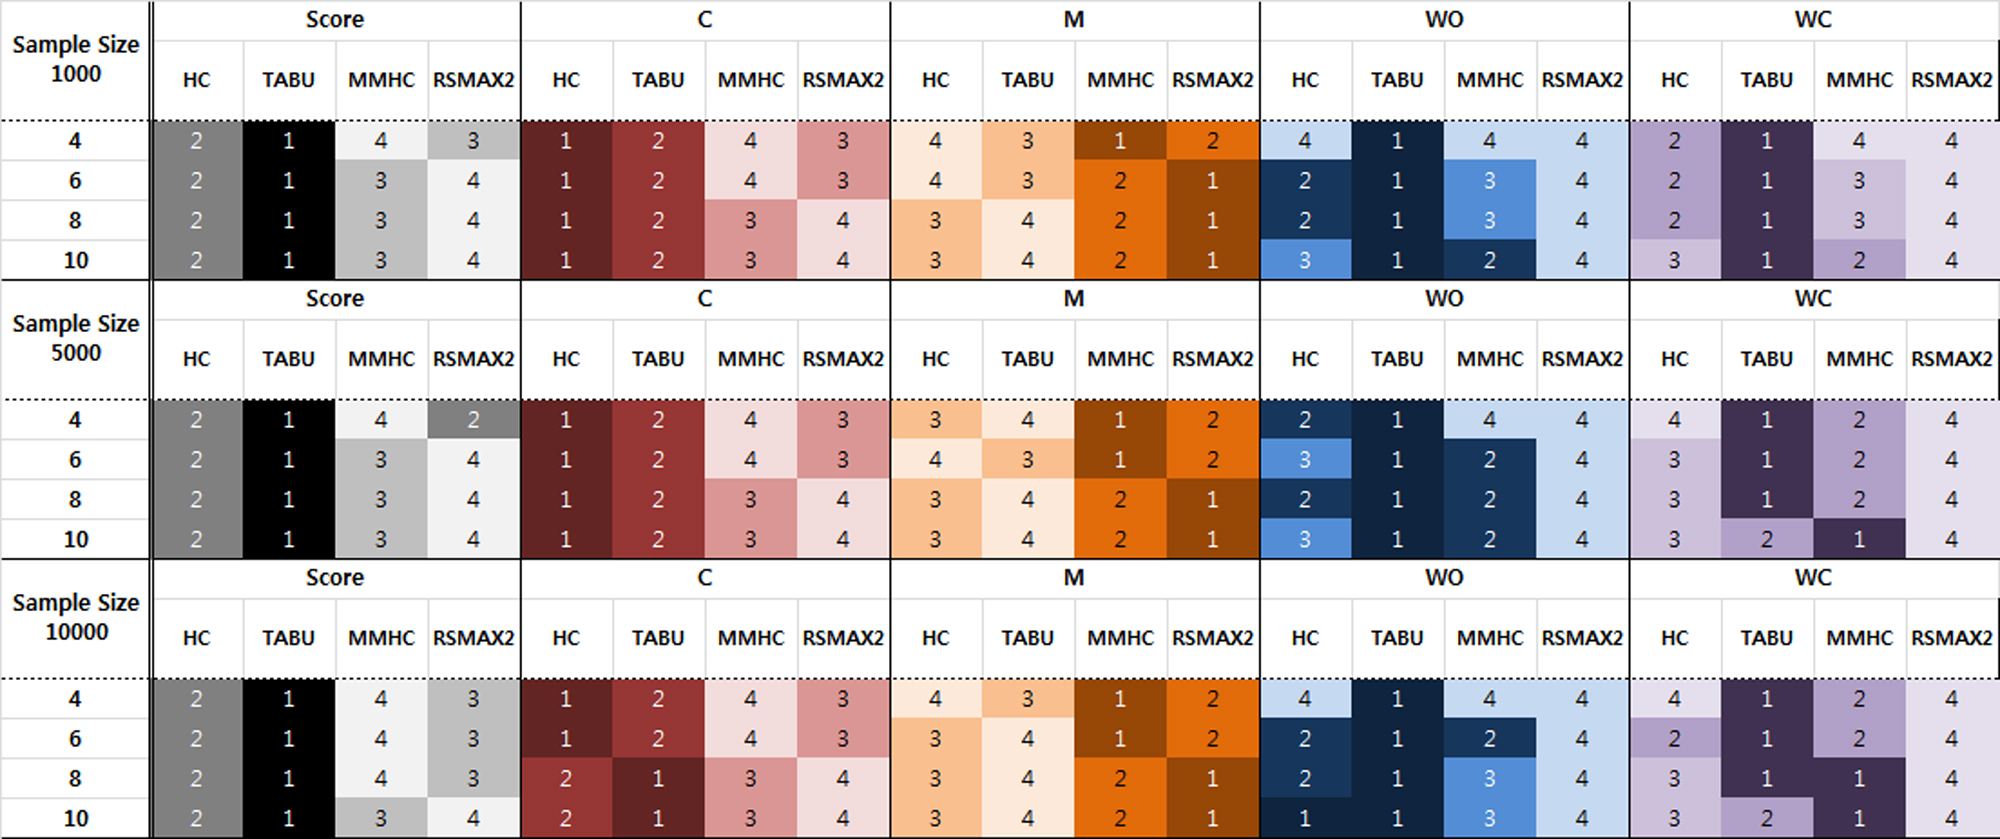
\includegraphics[height=130pt]{images/Result_Rhombus}
	\end{center}
}
\end{frame}


\section{결론}
\subsection{결론}
\begin{frame}
\frametitle{결론}
{\scriptsize{}
	Algorithm User가 판단해야할 문제	
	\begin{itemize}
		\item Score로 평가할 것인가, Model을 직접 비교하여 평가할 것인가?
		
		\item Model로 평가할 때, M, WO, WC에 대한 가중치는?
	\end{itemize}
}
\end{frame}


\begin{frame}
\frametitle{결론}
{\scriptsize{}
	bnlearn 패키지에서 제공하는, Score-Based Algorithm과 Hybrid Algorithm을 집중 비교해 본 결과 다음과 같은 결론을 내일 수 있었다.

	\begin{itemize}	
		\item "Score가 무엇이 더 높은가?", "Correct Arcs가 무엇이 더 많은가?" 어떤 것으로 비교해도 Score-Based 알고리즘(HC, TABU)가 Hybrid 알고리즘(MMHC, RSMAX2)보다 좋게 나타났다.
	
		\item 그러나 Score-Based 알고리즘을 적용했을 때, Wrongly Oriented and Connected Arcs도 많이 나타났다.
		
		{}\		
		
		특히 HC와 TABU만을 놓고 보면, TABU가 score는 더 좋지만, 학습된 모형을 보면 WO, WC 비중이 압도적으로 높았다.
		
		{}\		
		
		만일 학습된 결과 WO, WC가 많은 것이 C가 적은 것보다 문제가 되는 분야라면, Hybrid Algorithm을 선택하는 것도 방법이 될 수 있다.
	\end{itemize}	
}
\end{frame}


\begin{frame}
\frametitle{결론}
{\scriptsize{}
	bnlearn 패키지에서 제공하는, Score-Based Algorithm과 Hybrid Algorithm을 집중 비교해 본 결과 다음과 같은 결론을 내일 수 있었다.

	\begin{itemize}	
		\item Topology별로	???
		\item Sample Size별로	??
		\item Node 개수별로	??
	\end{itemize}	
}
\end{frame}

\subsection{Discussion}
\begin{frame}
\frametitle{Discussion}
{\scriptsize{}

	(컴퓨팅 시간을 기다릴 인내심만 있다면...)
	
	\begin{itemize}
		\item Topology의 Node 개수를 더 늘려볼 필요도 있다.
	
		\item 다른 Algorithm을 적용하여, Sample Size를 더 적게하여, Cardinality를 증가시켜 추가 실험을 진행해 볼 수 있다.

		\item 서로 다른 Topology를 결합하여 비교 분석 할 수도 있다.

		\item Bayesian Network Data Generator의 R 패키징 완성
		
		\item 확률 관계를 정의할 때 확률값을 U(0,1) 사이의 값에서 임의로 주었는데, 이 확률값을 "순차적"으로 준 것과의 관계를 알아볼 수도 있다.
	\end{itemize}
	
	{}\	
	
	다른 연구 과제
	
	\begin{itemize}	
		\item  Bayesian Network를 이용하여 Missing Value를 컨트롤
		
		(이 때 Bayesian Network Data Generator를 적극 활용할 수 있다.)
		
			~~~~~1. 배경 지식을 바탕으로 만든 모형을 이용하여 데이터를 생성하는 방법
			
			~~~~~2. Missing이 없는 부분을 이용하여 먼저 구조학습을 한 후, 학습된 모형으로 데이터를 생성하는 방법
			
			~~~~~3. 조건부가 Missing인 부분에 대한 조건부 확률관계를 표현하는 Node를 추가로 생성하는 방법			
	\end{itemize}
}
\end{frame}

\end{document}

